% ============================================================================
% Final presentation (Beamer, metropolis theme, 16:9). Numbers identical to main_v2.tex.
% Build: pdflatex presentation.tex (twice)
% ============================================================================
\documentclass[aspectratio=169,11pt]{beamer}
\usetheme[progressbar=frametitle,numbering=fraction,sectionpage=progressbar]{metropolis}
\usepackage[utf8]{inputenc}
\usepackage[T1]{fontenc}
\usepackage{booktabs}
\usepackage{graphicx}
\graphicspath{{./}{figures/}}

% ---- colours (navy / teal / amber) -----------------------------------------
\definecolor{navy}{HTML}{1F3A5F}
\definecolor{teal}{HTML}{1F7A7A}
\definecolor{amber}{HTML}{C26A00}
\definecolor{soft}{HTML}{F4F6F9}
\setbeamercolor{normal text}{fg=navy!90!black, bg=white}
\setbeamercolor{frametitle}{bg=navy, fg=white}
\setbeamercolor{progress bar}{fg=amber, bg=navy!25}
\setbeamercolor{title separator}{fg=amber}
\setbeamercolor{alerted text}{fg=amber}
\setbeamercolor{block title}{bg=navy!12, fg=navy}
\setbeamercolor{block body}{bg=soft}
\setbeamertemplate{itemize item}{\color{amber}$\blacktriangleright$}
\setbeamertemplate{itemize subitem}{\color{teal}--}

\newcommand{\bignum}[2]{%
  \begin{center}{\fontsize{30}{32}\selectfont\bfseries\color{amber}#1}\\[3pt]{\small\color{navy}#2}\end{center}}
\newcommand{\hint}[1]{{\footnotesize\color{navy!65}#1}}

\title{A Multimodal Framework for Agricultural Drought\\Monitoring and Prediction}
\subtitle{Weather time series $\cdot$ Satellite imagery $\cdot$ UAV semantic segmentation}
\author{G.\ Aryan Rajesh (123CS0020) \quad M.\ Rovan (123CS0036) \quad M.\ Harsha Vardhan (123CS0044)}
\institute{Guide: Dr.\ M.\ Naresh Babu, Associate Professor, Dept.\ of CSE\\IIITDM Kurnool}
\date{November 2026}
\titlegraphic{\hfill
\includegraphics[height=1.5cm]{figures/logo.jpeg}}

\begin{document}

\maketitle

\begin{frame}{Outline}
  \tableofcontents
\end{frame}

% ============================================================================
\section{Problem and idea}

\begin{frame}{The problem}
  \begin{columns}[T]
    \column{0.55\textwidth}
    \begin{itemize}
      \item Rayalaseema farming depends on rain (\alert{kharif}) and stored soil water (\alert{rabi})
      \item Drought is \alert{declared late} by the government, often months after crops suffer
      \item Weather, satellite and drone studies are usually done \alert{separately}
    \end{itemize}
    \column{0.42\textwidth}
    \begin{block}{Our question}
      Can we \textbf{forecast} drought, \textbf{confirm} it on crops, and \textbf{measure} it on fields --- in both seasons?
    \end{block}
  \end{columns}
\end{frame}

\begin{frame}{Our idea: three modules, two seasons}
  \centering
  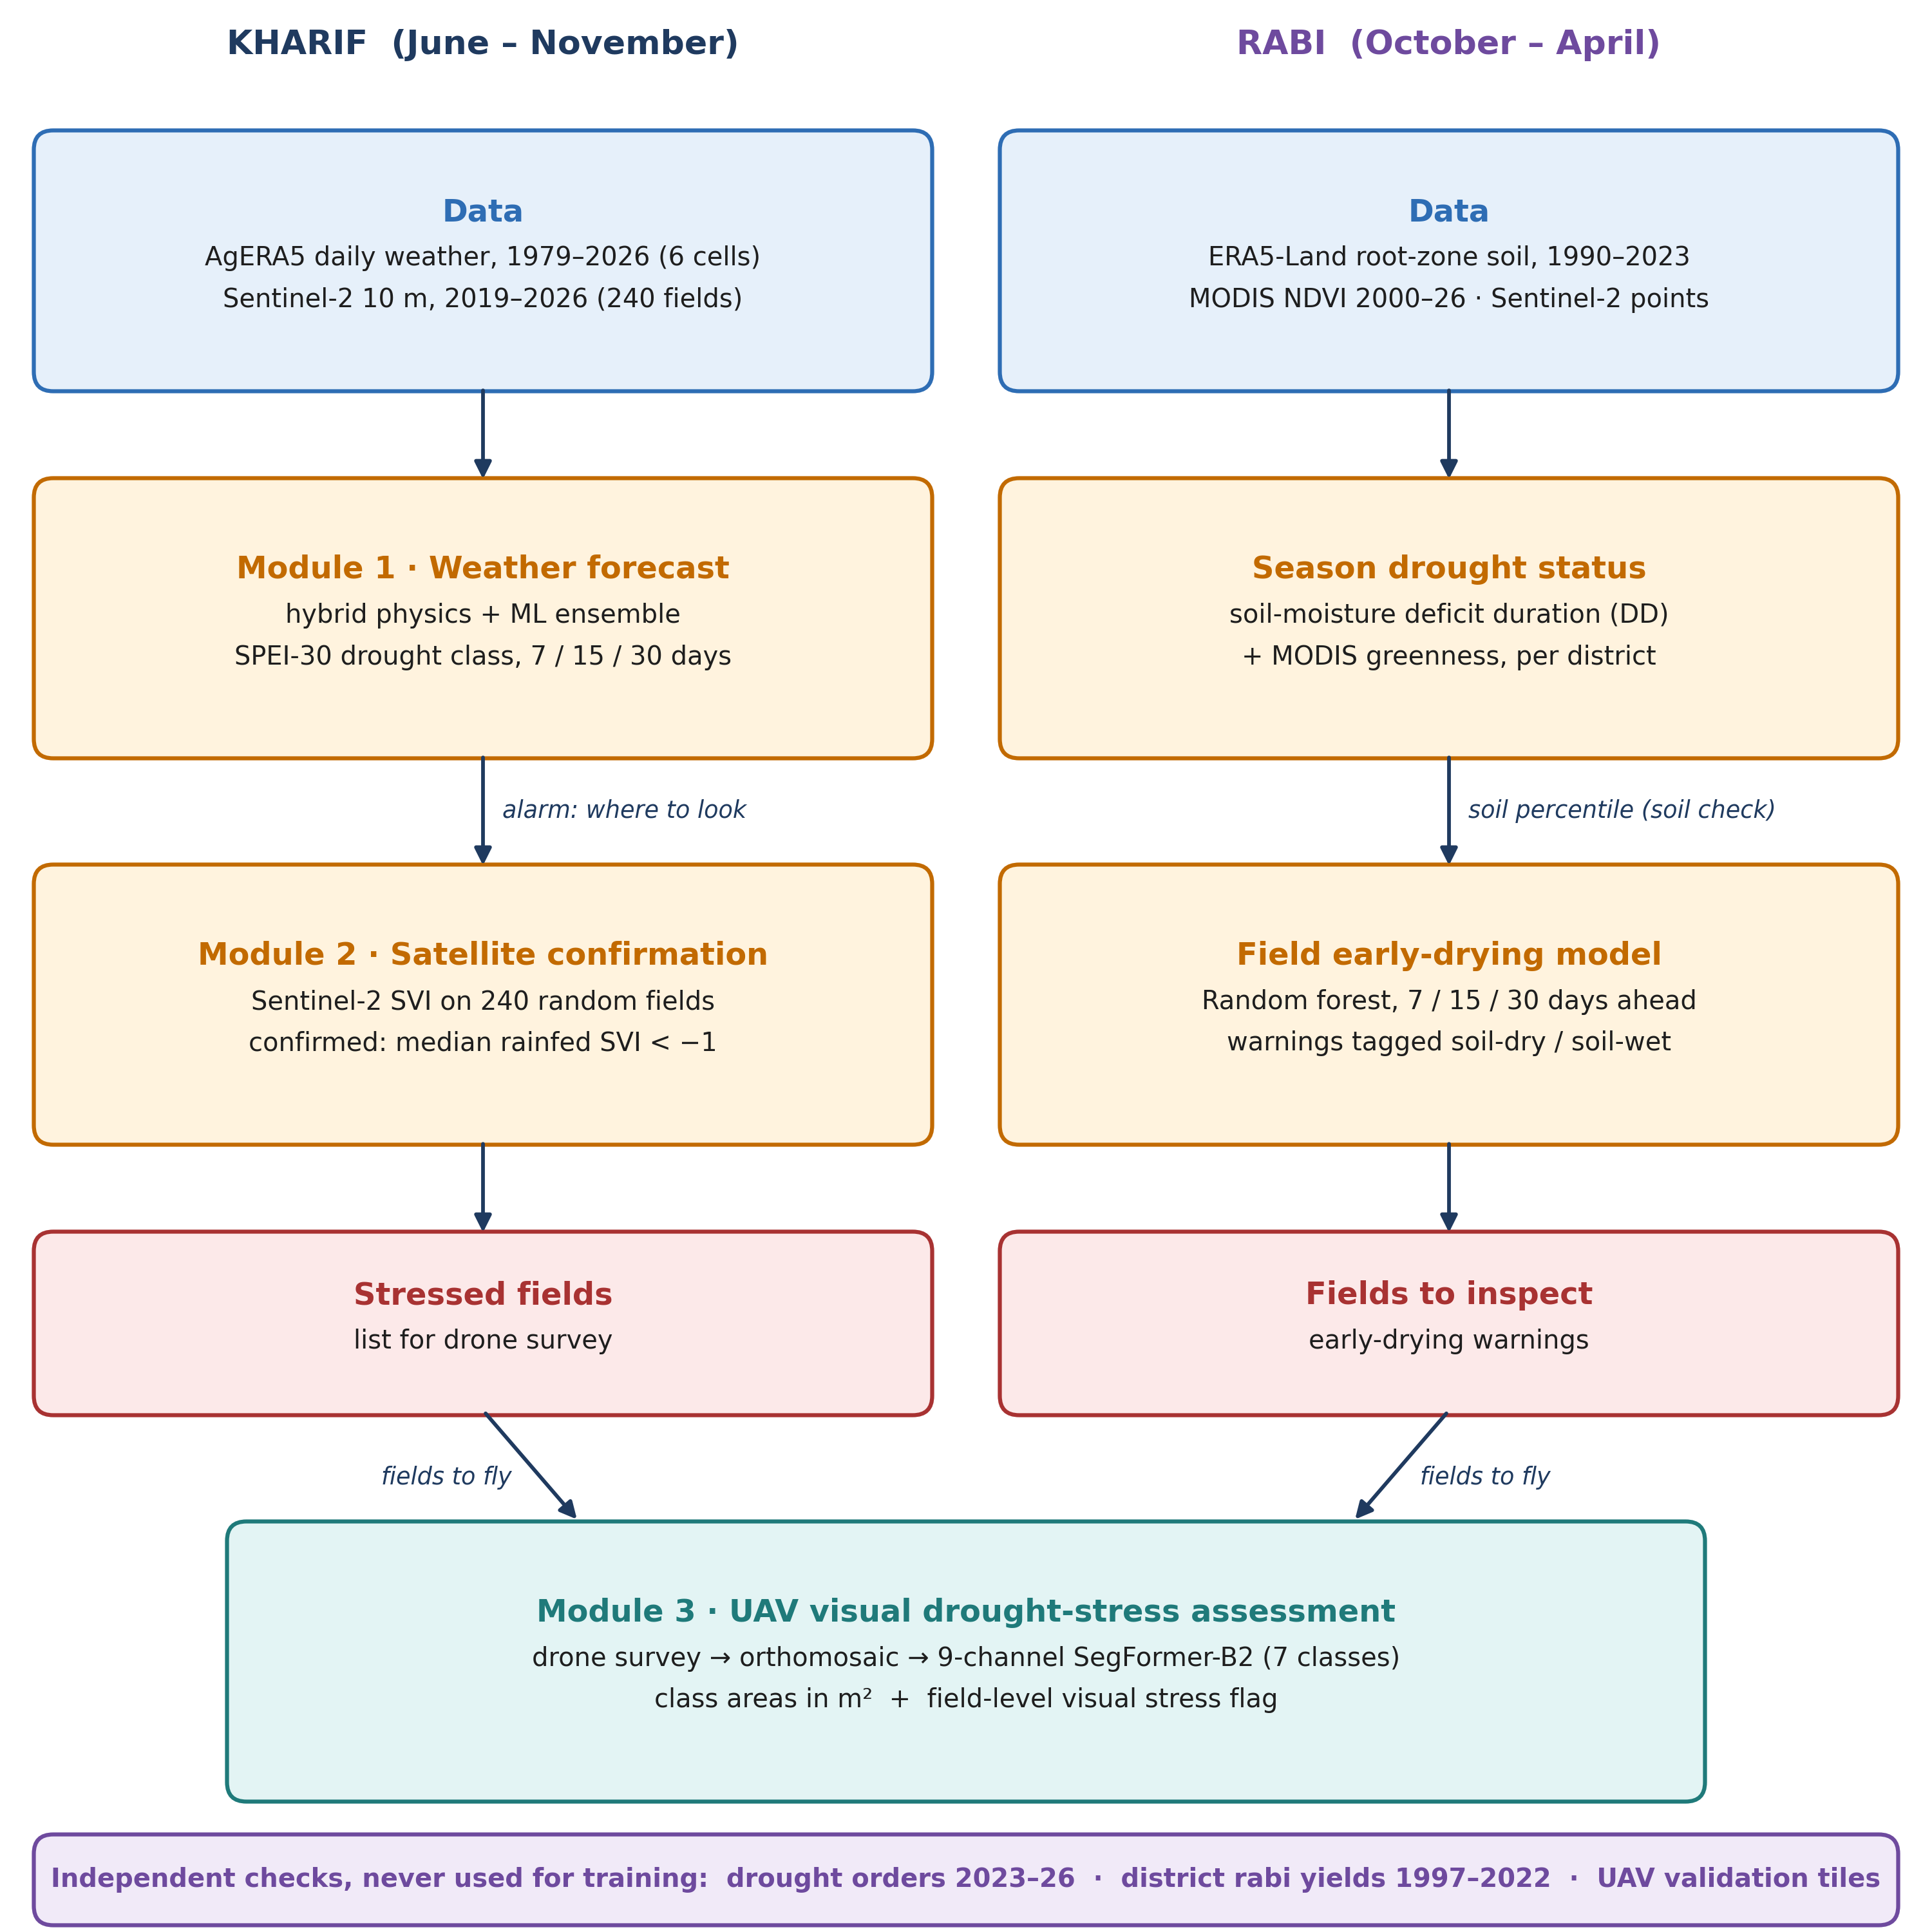
\includegraphics[height=0.82\textheight]{figures/v2_system.png}
\end{frame}

\begin{frame}{Study area and data}
  \begin{columns}[T]
    \column{0.42\textwidth}
    \textbf{8 sites}
    \begin{itemize}
      \item Kurnool (4 sites)
      \item Sri Sathya Sai (3 sites)
      \item Tumakuru, Karnataka (1 site)
    \end{itemize}
    \vspace{4pt}
    \hint{Nothing is simulated: all data are public or collected by the team.}
    \column{0.56\textwidth}
    \small
    \begin{tabular}{@{}ll@{}}
      \toprule
      \textbf{Data} & \textbf{Years} \\
      \midrule
      Daily weather (AgERA5) & 1979--2026 \\
      Sentinel-2 satellite, 10\,m & 2019--2026 \\
      Soil moisture (ERA5-Land) & 1990--2023 \\
      MODIS greenness, 250\,m & 2000--2026 \\
      District crop yields & 1997--2022 \\
      Drone surveys (14 orthomosaics) & Nov 2025 -- Jan 2026 \\
      Government drought orders & 2023--2026 \\
      \bottomrule
    \end{tabular}
  \end{columns}
\end{frame}

% ============================================================================
\section{Kharif module: weather + satellite}

\begin{frame}{Module 1: weather forecast --- how it works}
  \centering
  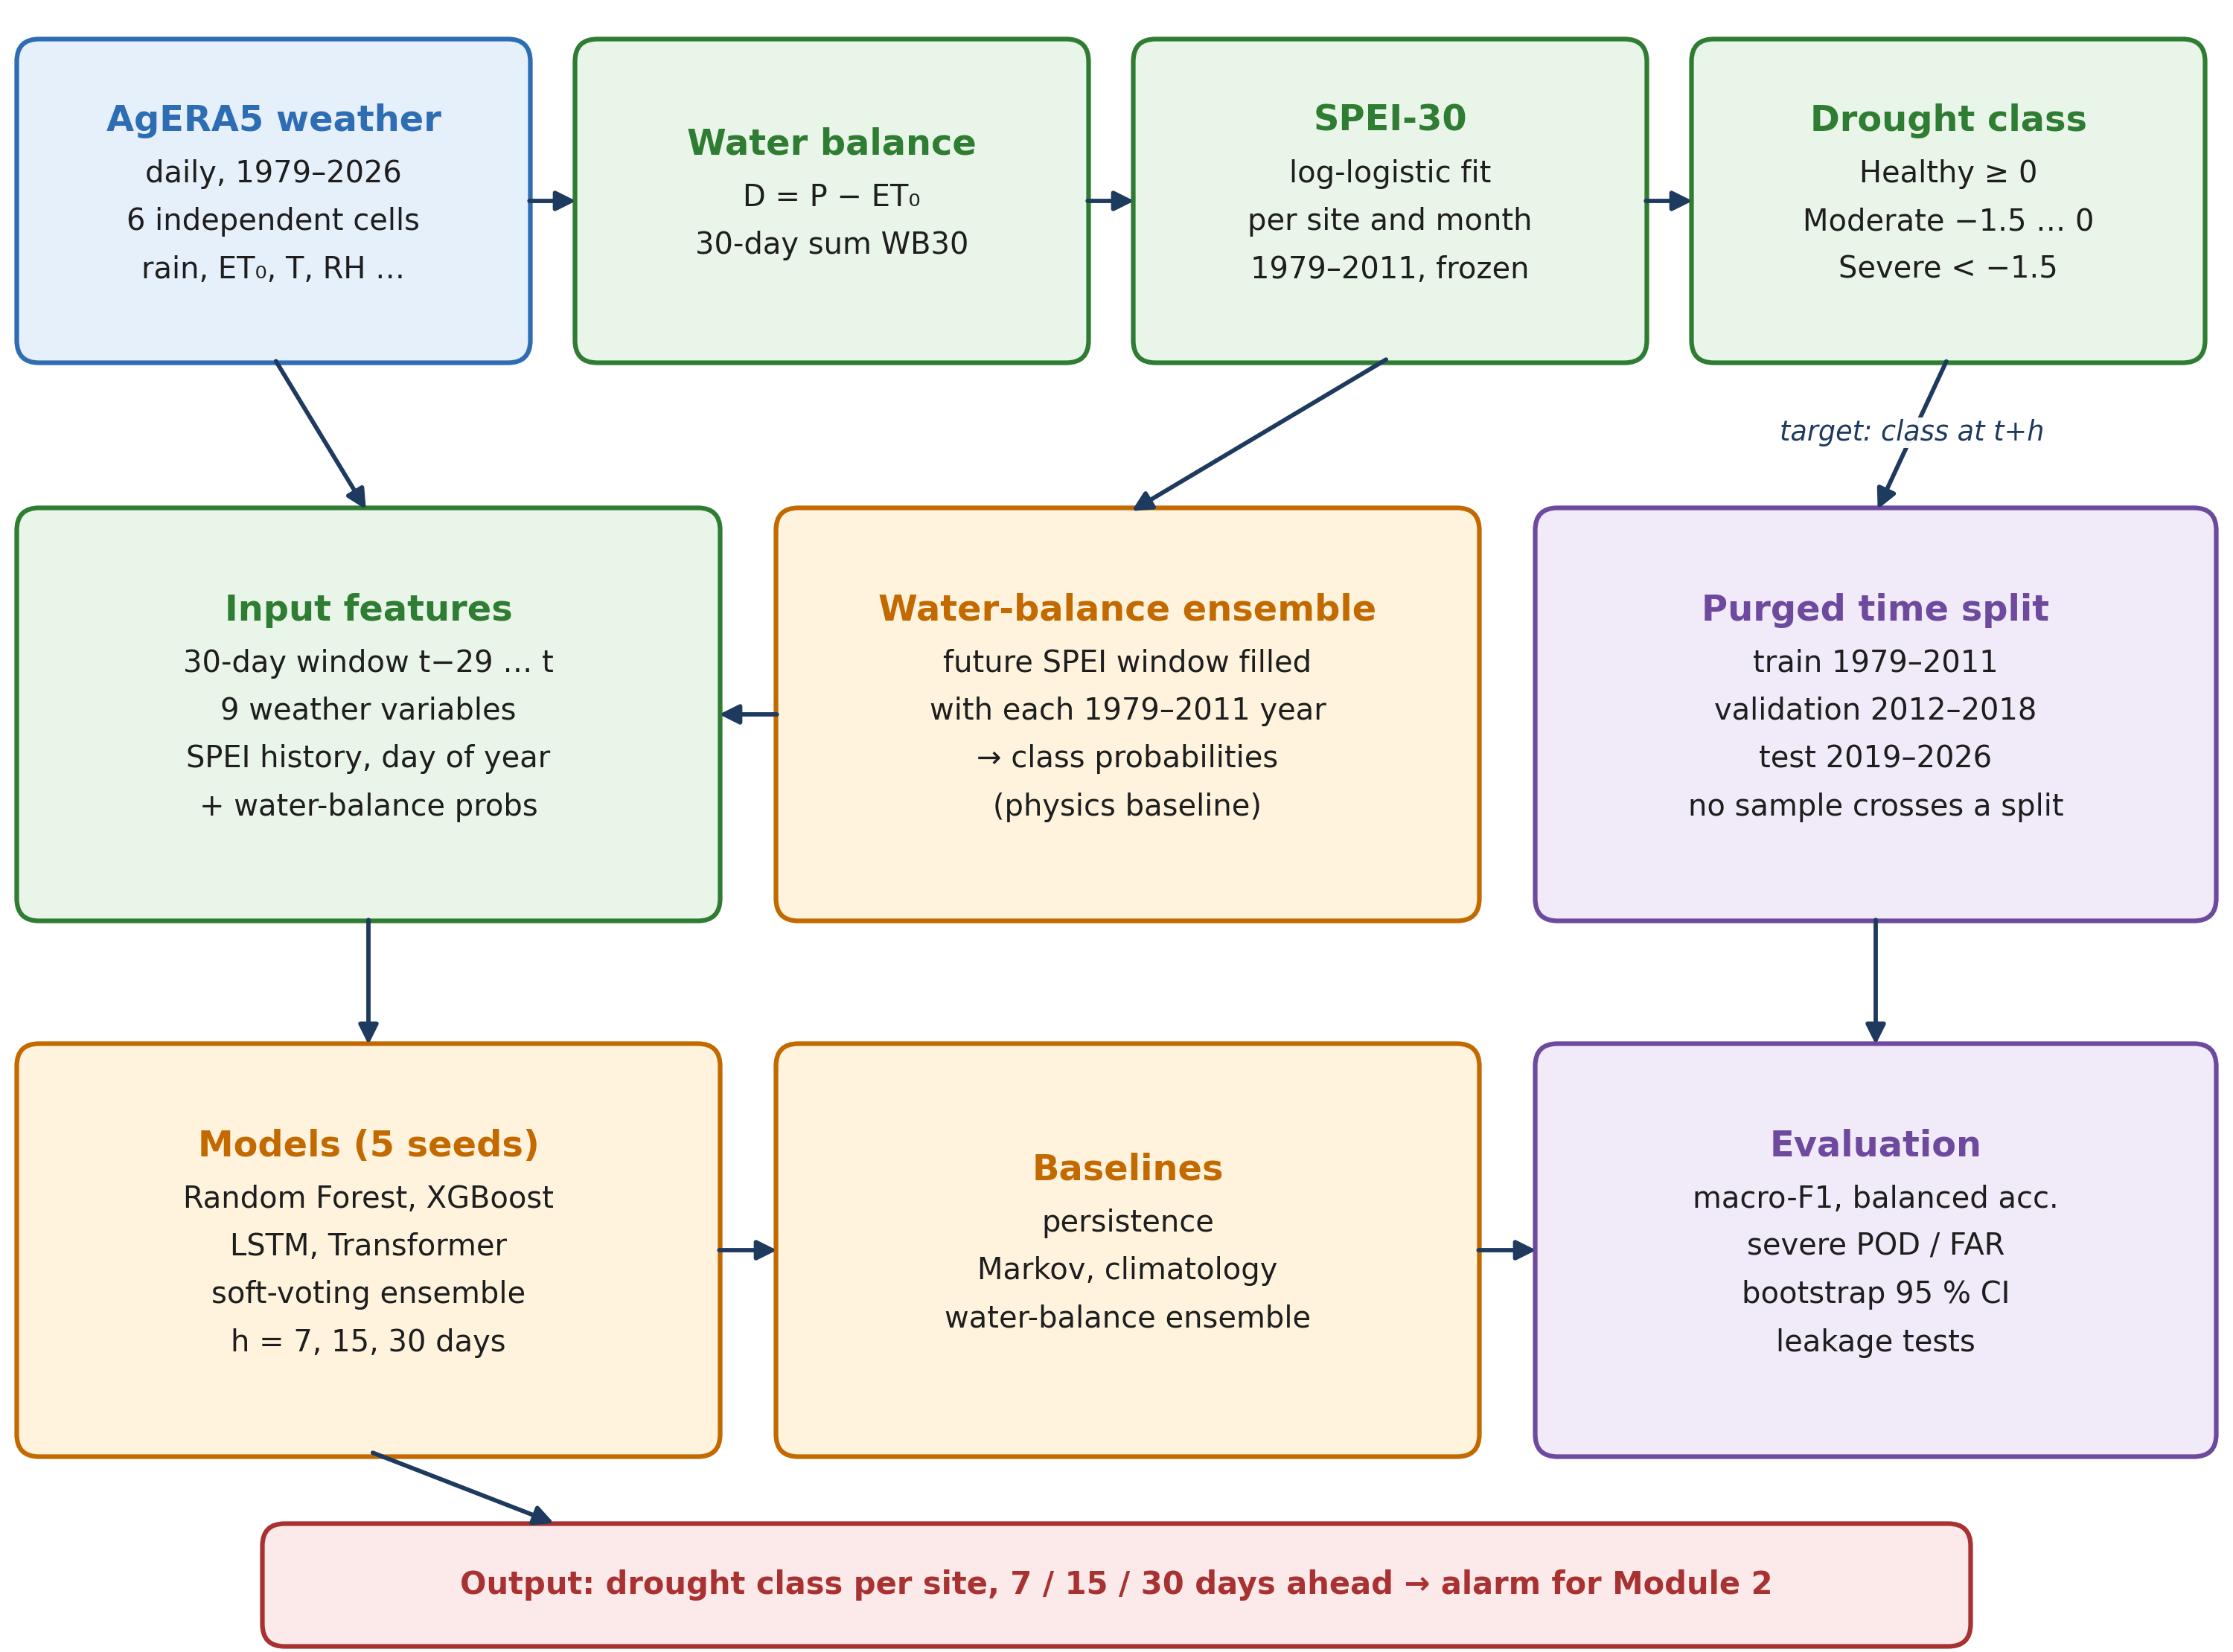
\includegraphics[height=0.66\textheight]{figures/v2_weather.png}\\[2pt]
  \hint{Drought class from SPEI-30 (water balance). Physics (water balance of past years) + machine learning.}
\end{frame}

\begin{frame}{Module 1: results (test years 2019--2026)}
  \begin{columns}[c]
    \column{0.36\textwidth}
    \bignum{0.819}{macro-F1, 7 days ahead\\(persistence 0.662)}
    \bignum{80\,\%}{of severe-drought days\\caught 7 days ahead}
    \column{0.62\textwidth}
    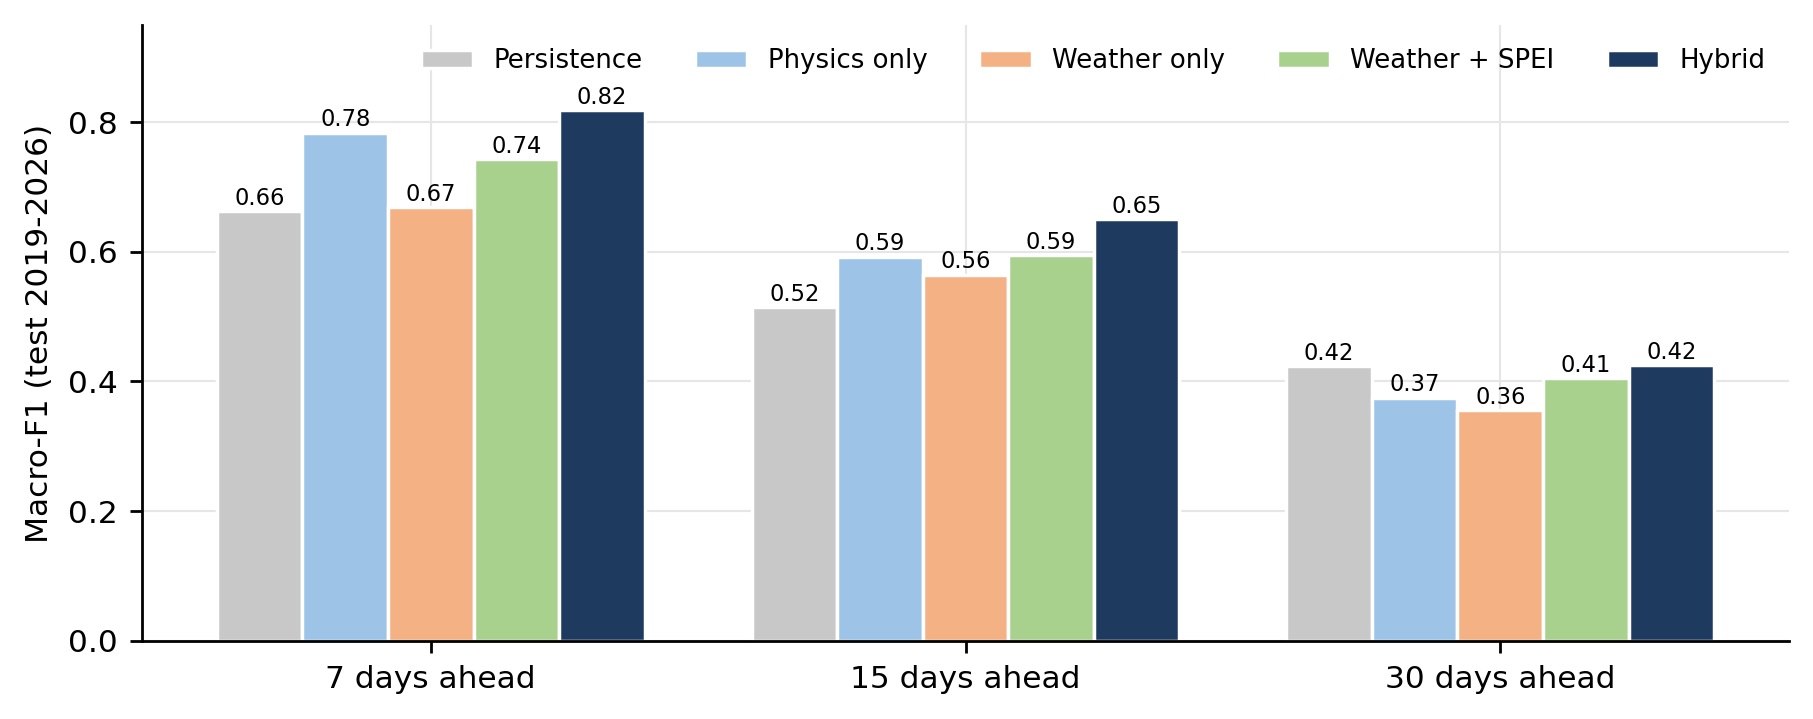
\includegraphics[width=\textwidth]{figures/res_w_bars.png}\\
    \hint{Physics input gives the biggest gain. At 30 days nothing beats persistence --- reported honestly.}
  \end{columns}
\end{frame}

\begin{frame}{Module 2: satellite confirmation --- how it works}
  \centering
  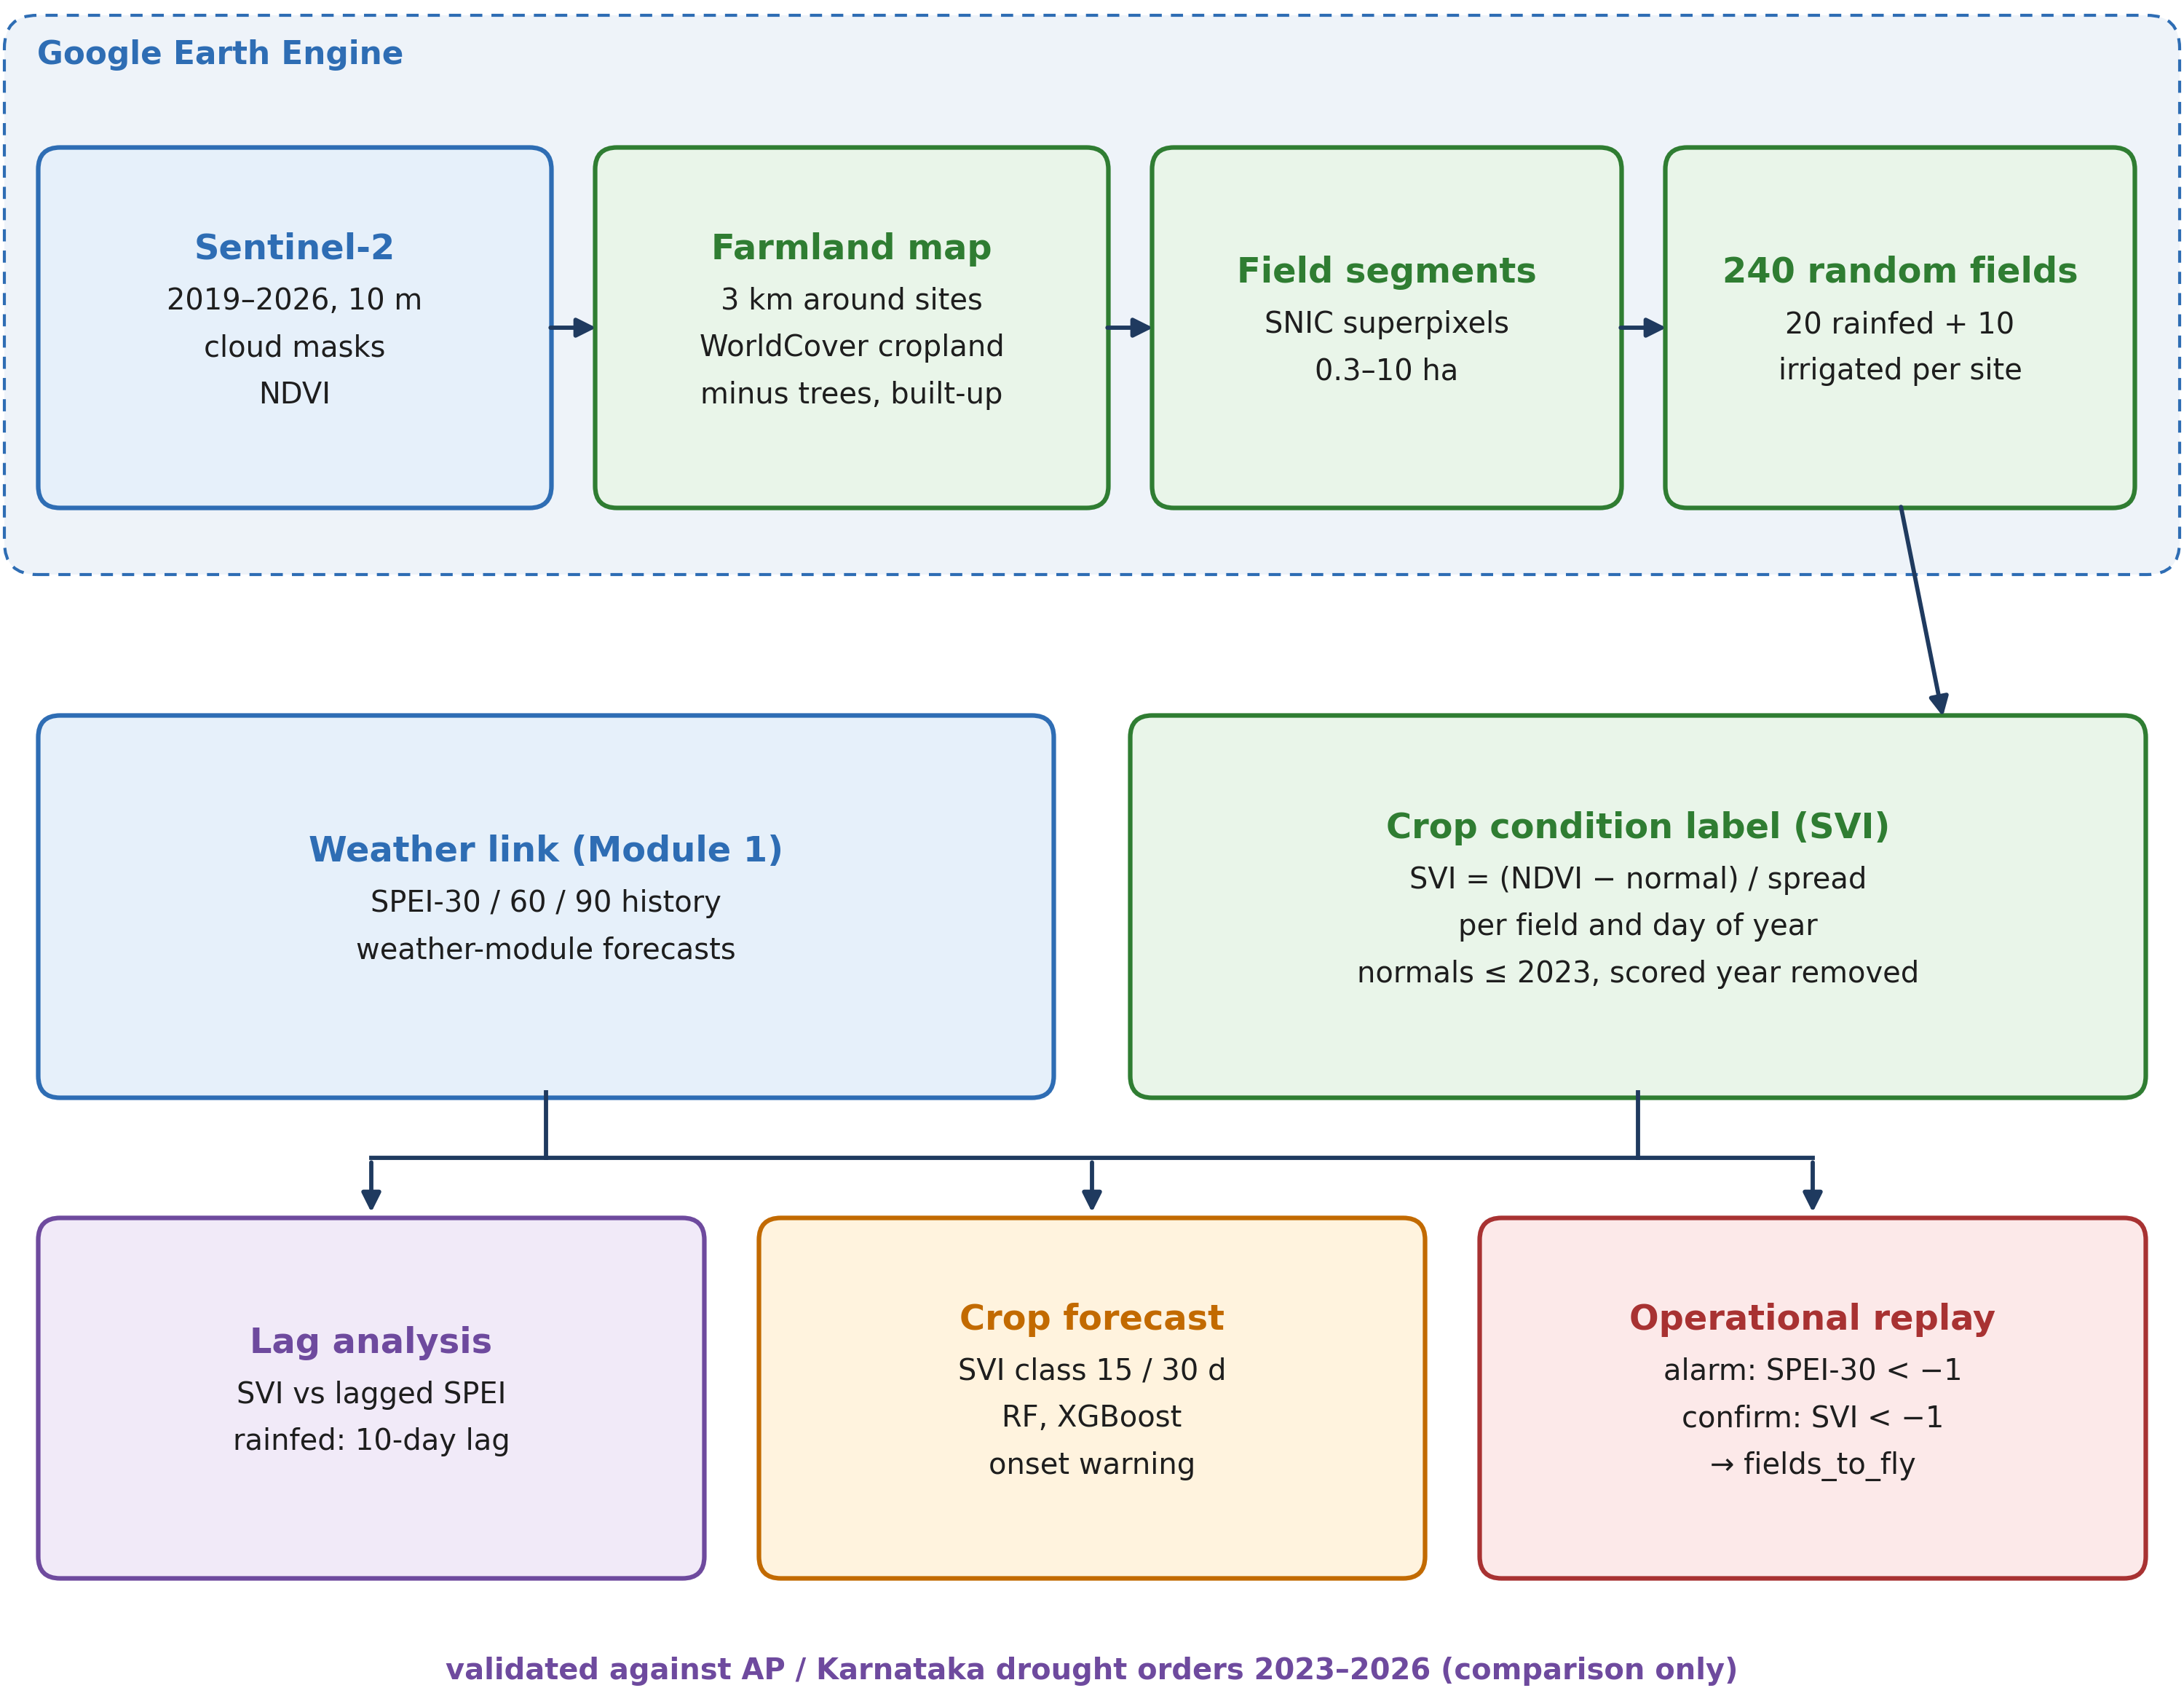
\includegraphics[height=0.68\textheight]{figures/v2_satellite.png}\\[2pt]
  \hint{240 random fields; crop condition = Standardized Vegetation Index (SVI).}
\end{frame}

\begin{frame}{Module 2: results}
  \begin{columns}[c]
    \column{0.32\textwidth}
    \bignum{10 days}{crops follow weather drought\\(rainfed fields)}
    \column{0.32\textwidth}
    \bignum{0.76}{AUC: which fields will\\become stressed in 15 days}
    \column{0.32\textwidth}
    \bignum{0.45}{correlation on unseen\\years 2024--2026}
  \end{columns}
  \vspace{6pt}
  \begin{itemize}
    \item A weather alarm is a good signal for \emph{where to look} with the satellite
  \end{itemize}
\end{frame}

\begin{frame}{Kharif chain vs government drought orders (2023--2026)}
  \begin{columns}[c]
    \column{0.46\textwidth}
    \centering
    \begin{tabular}{@{}lcc@{}}
      \toprule
      \textbf{Official} & \textbf{Confirmed} & \textbf{Before order} \\
      \midrule
      Severe & \alert{\textbf{9 / 9}} & 5 / 9 \\
      Moderate & 3 / 6 & 3 / 6 \\
      Not declared & 1 / 11 & (false alarm) \\
      \bottomrule
    \end{tabular}\\[8pt]
    \hint{Replayed with real data delays (weather 7 days, satellite 2 days late).}
    \column{0.52\textwidth}
    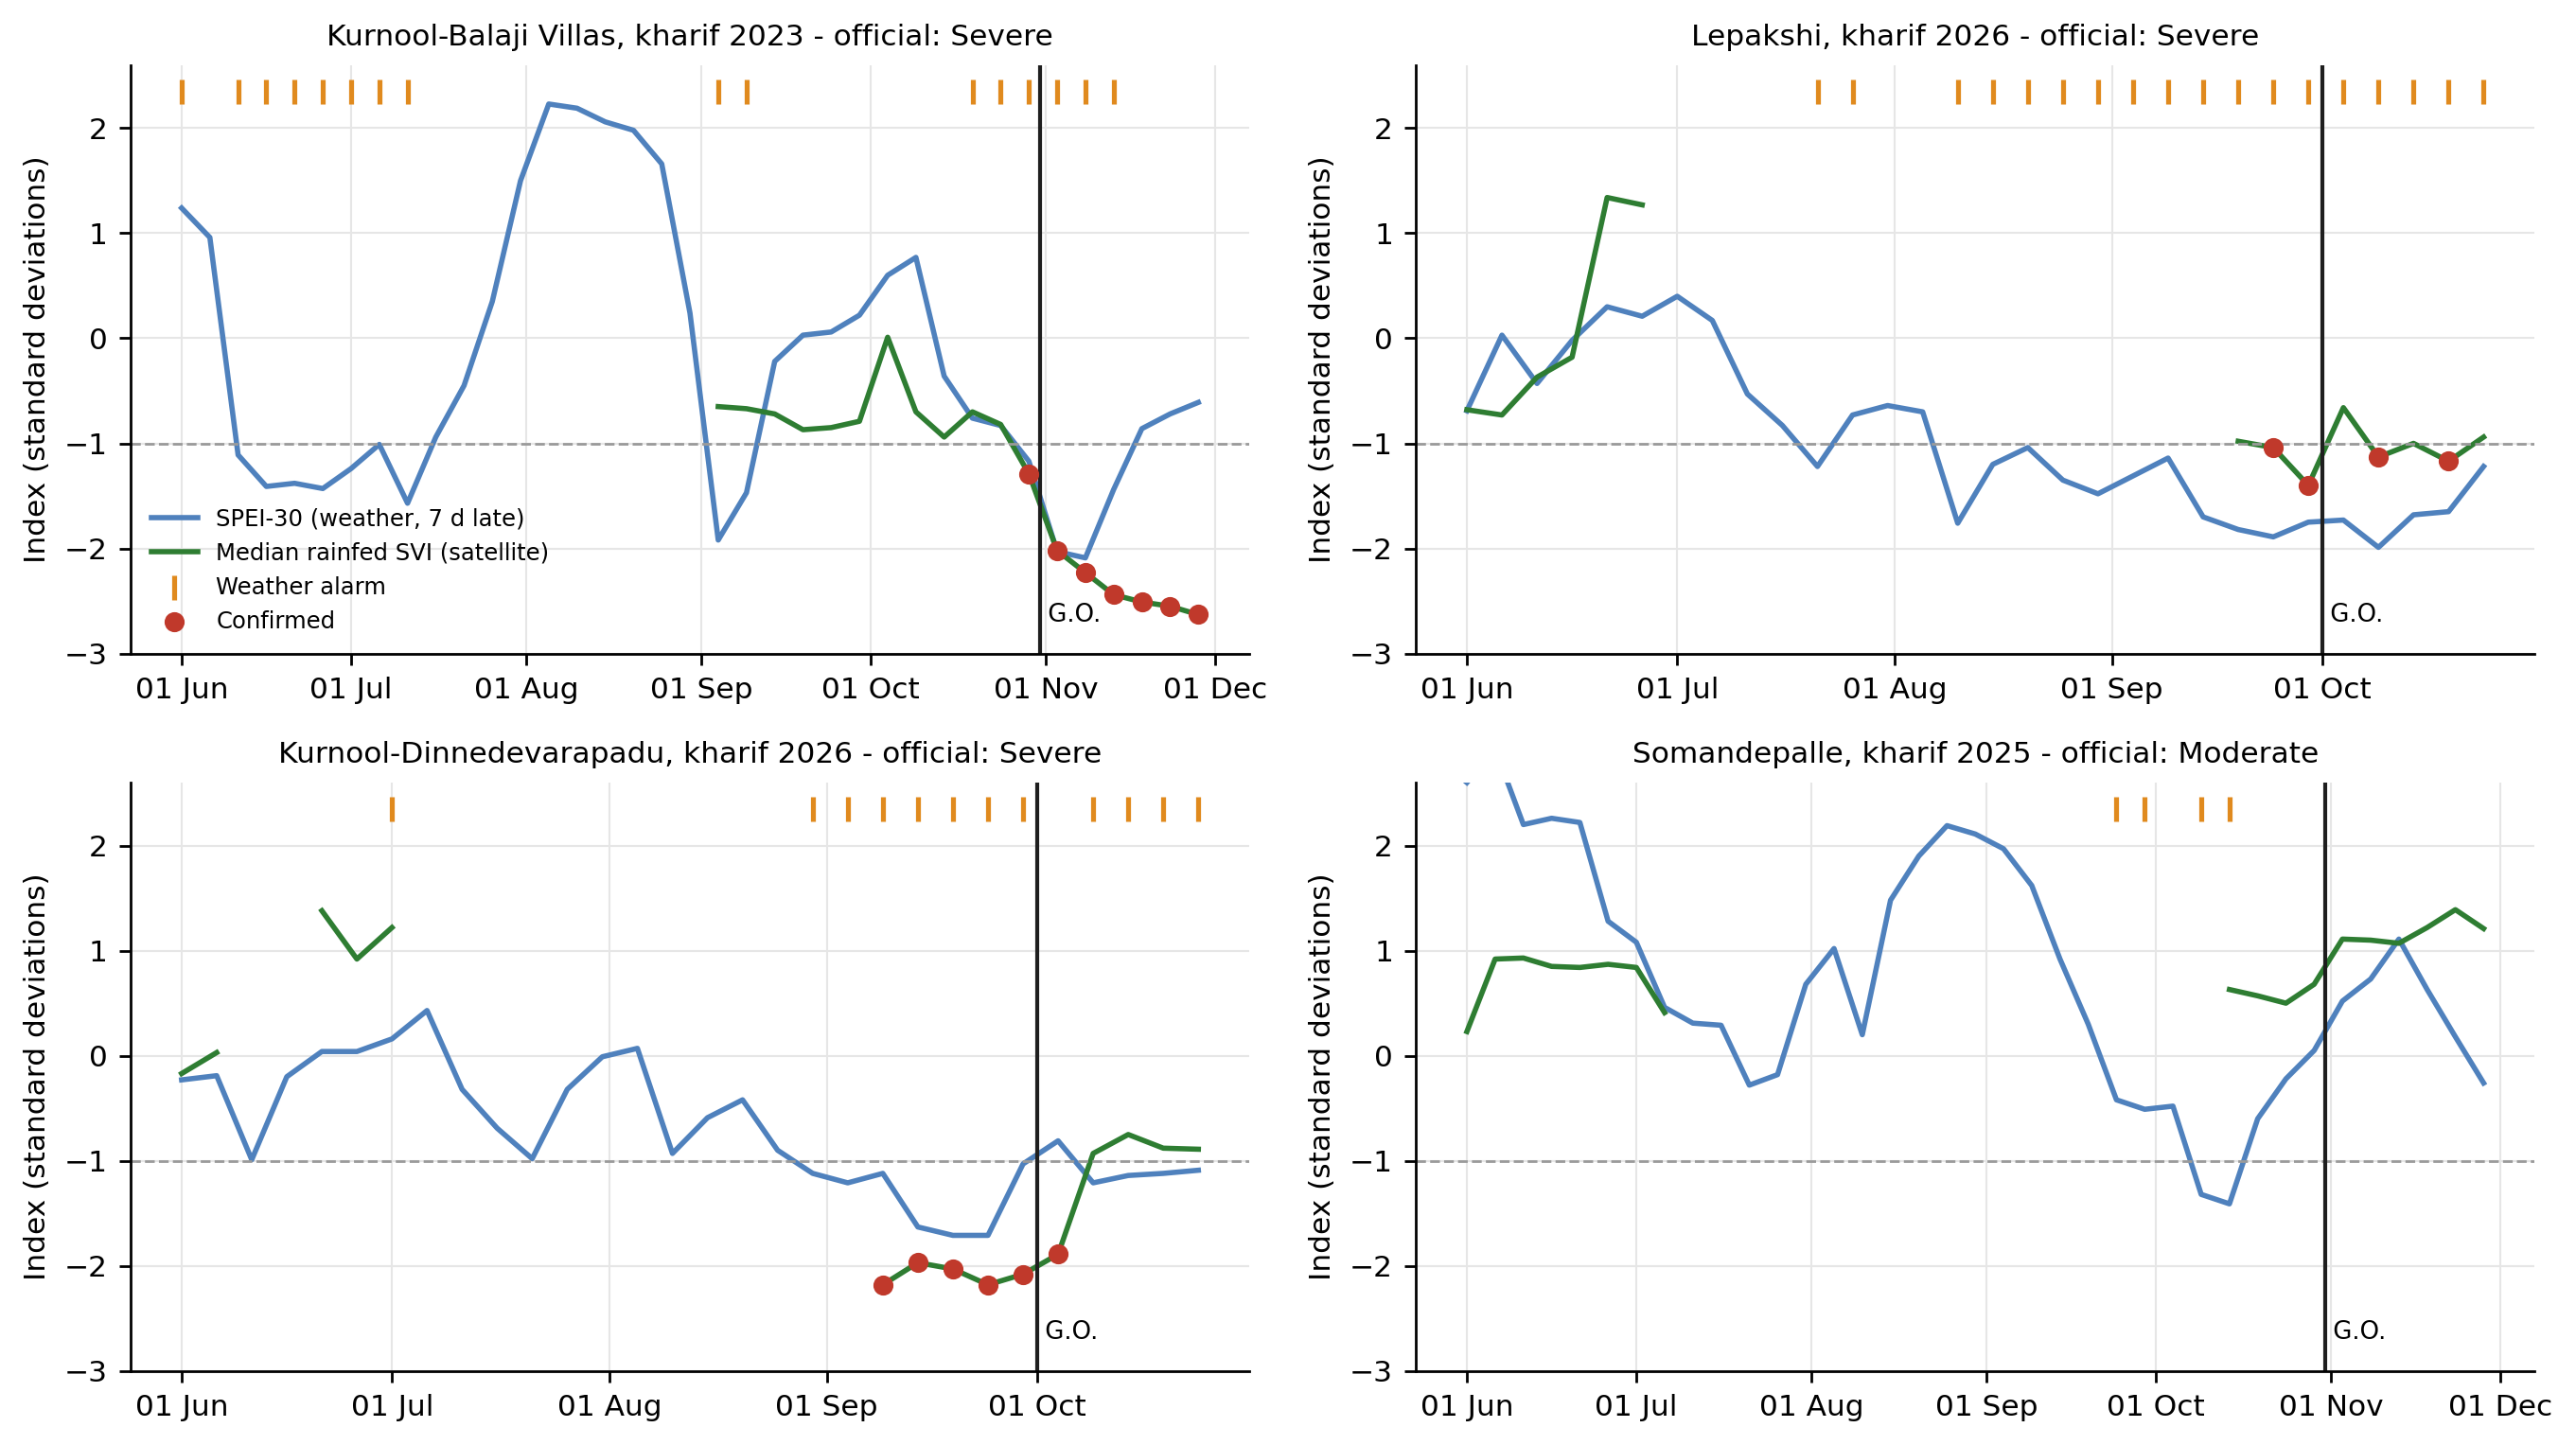
\includegraphics[width=\textwidth]{figures/res_s_cases.png}
  \end{columns}
\end{frame}

% ============================================================================
\section{Rabi module}

\begin{frame}{Why rabi needs its own module}
  \begin{itemize}
    \item Rabi crops grow on \alert{stored soil water}, not rain
    \item Rain-based drought indices miss this
    \item The kharif chain confirmed \alert{0 of 4} severe rabi droughts
  \end{itemize}
  \vspace{6pt}
  \begin{block}{Our approach}
    Measure \textbf{root-zone soil moisture} and check it against \textbf{real crop yields} (not against a few government orders).
  \end{block}
\end{frame}

\begin{frame}{Rabi module --- how it works}
  \centering
  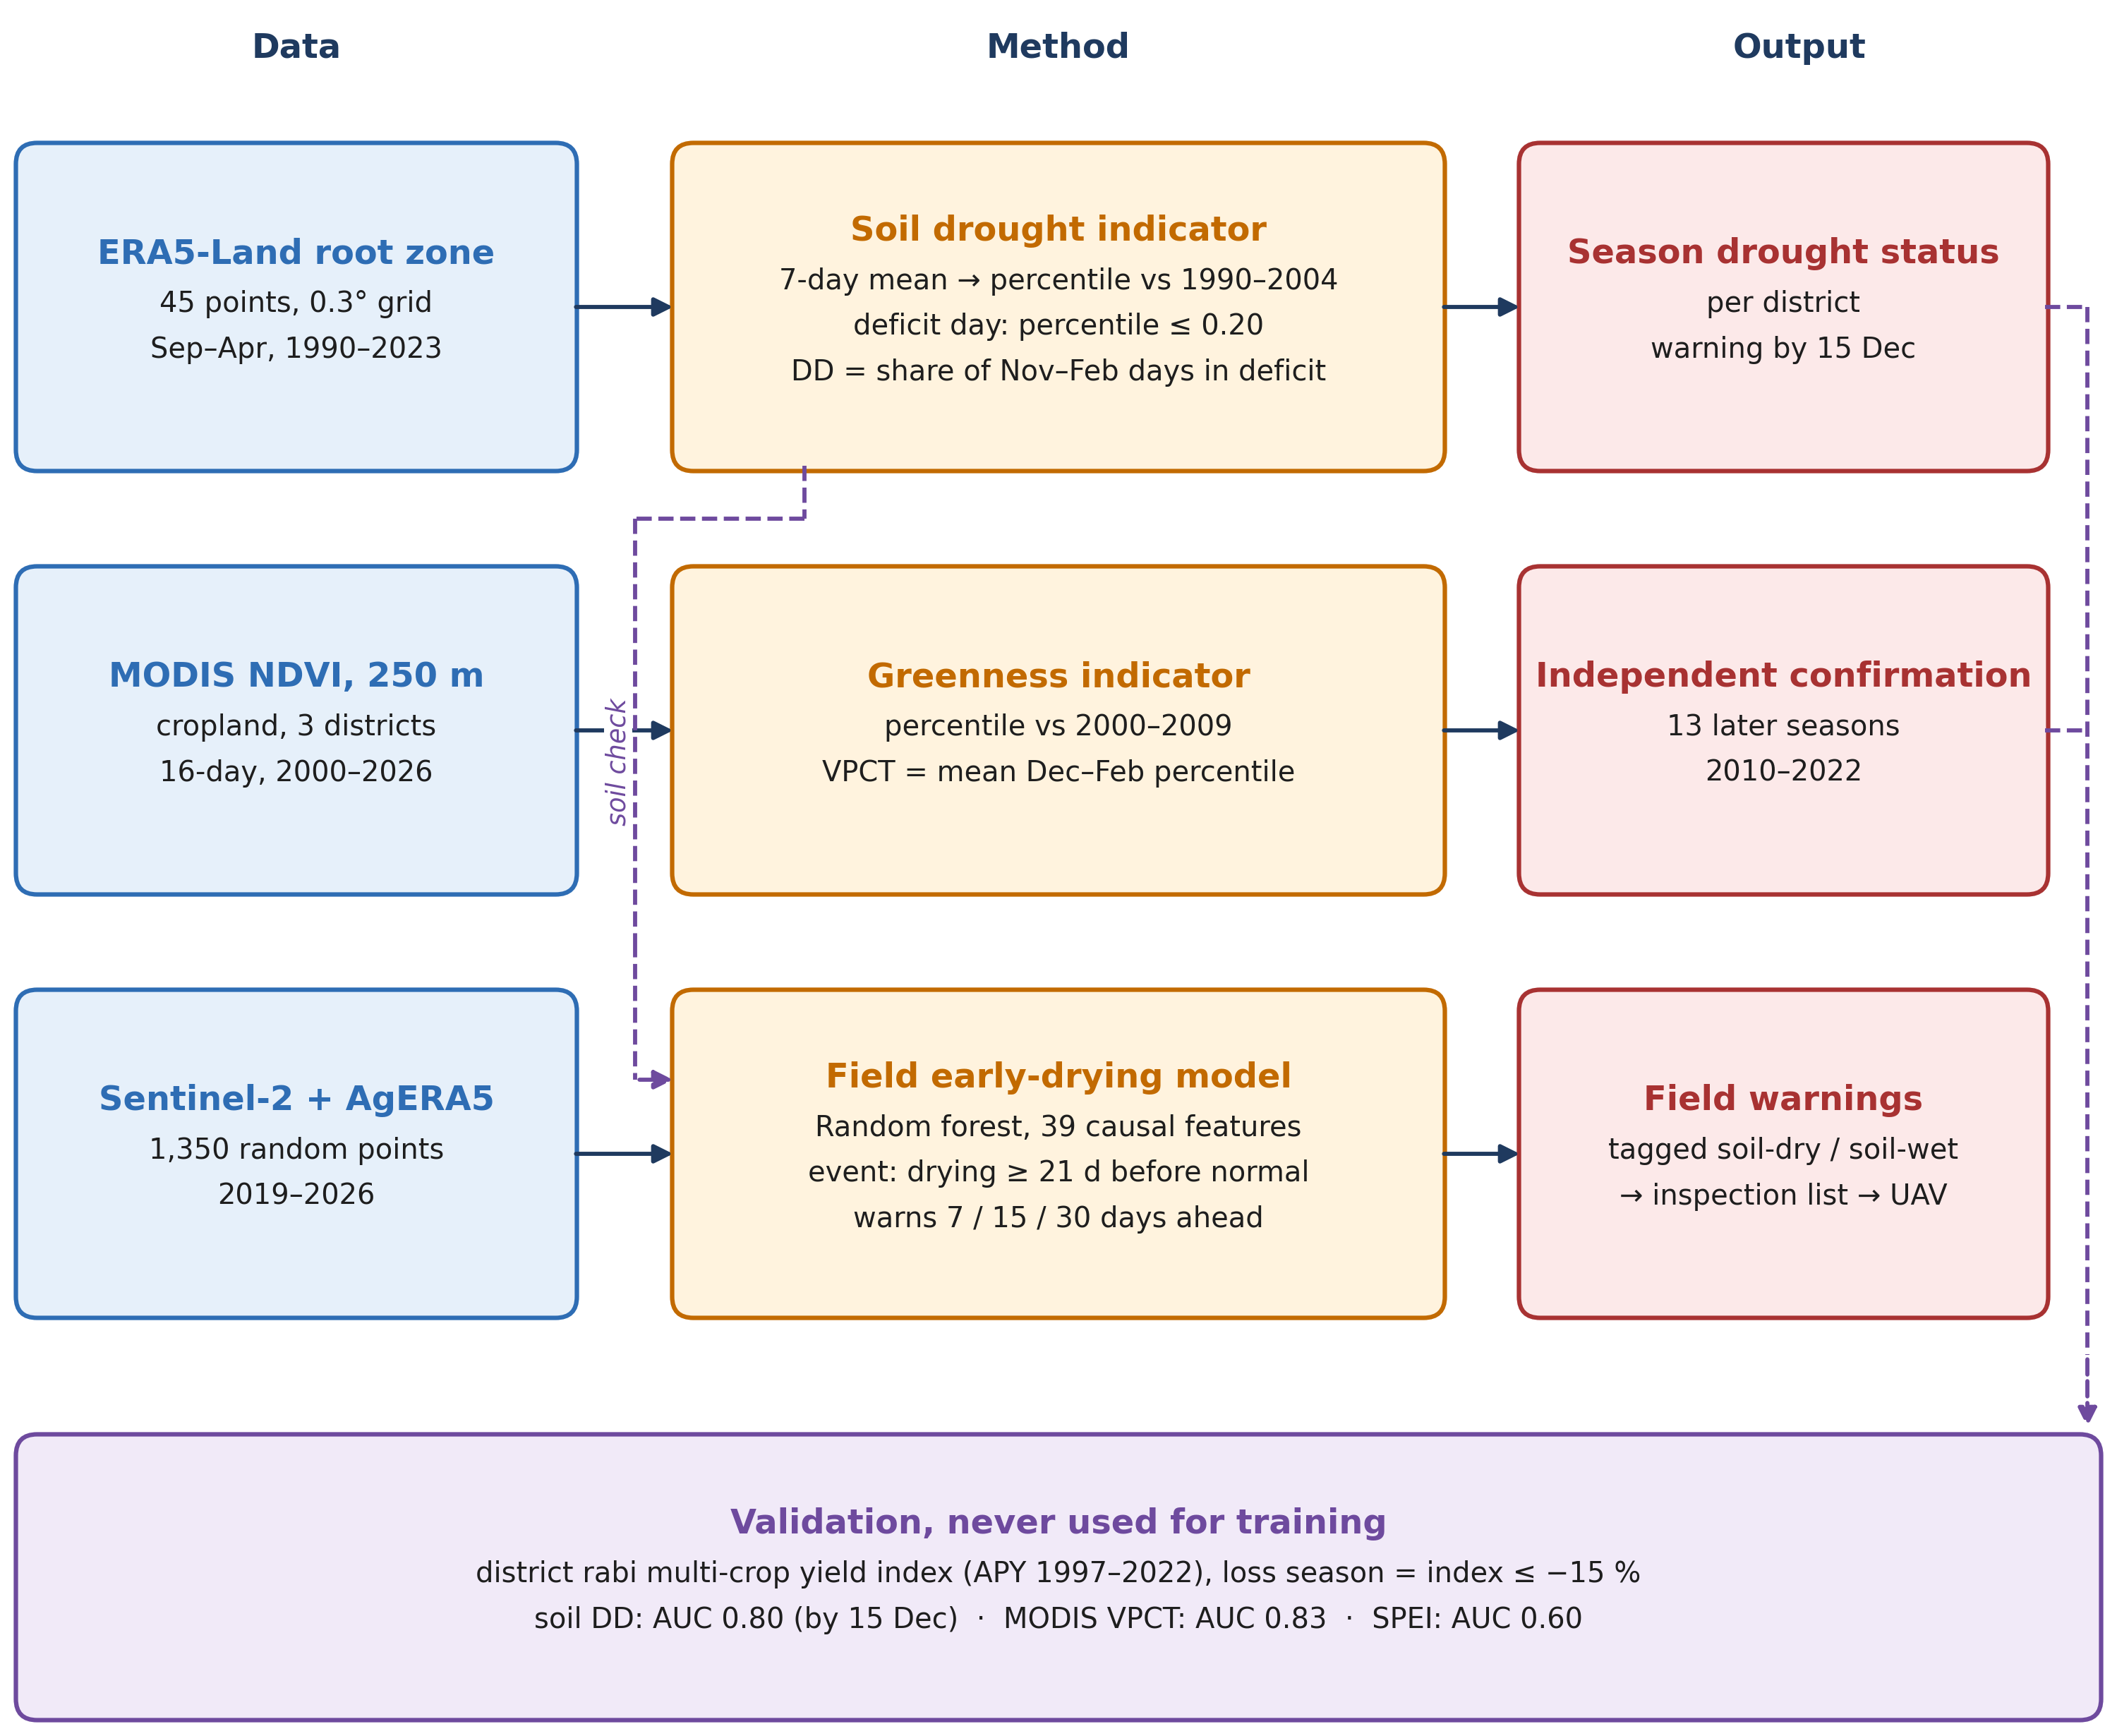
\includegraphics[height=0.82\textheight]{figures/v2_rabi.png}
\end{frame}

\begin{frame}{Rabi results: soil and greenness detect crop-loss seasons}
  \centering
  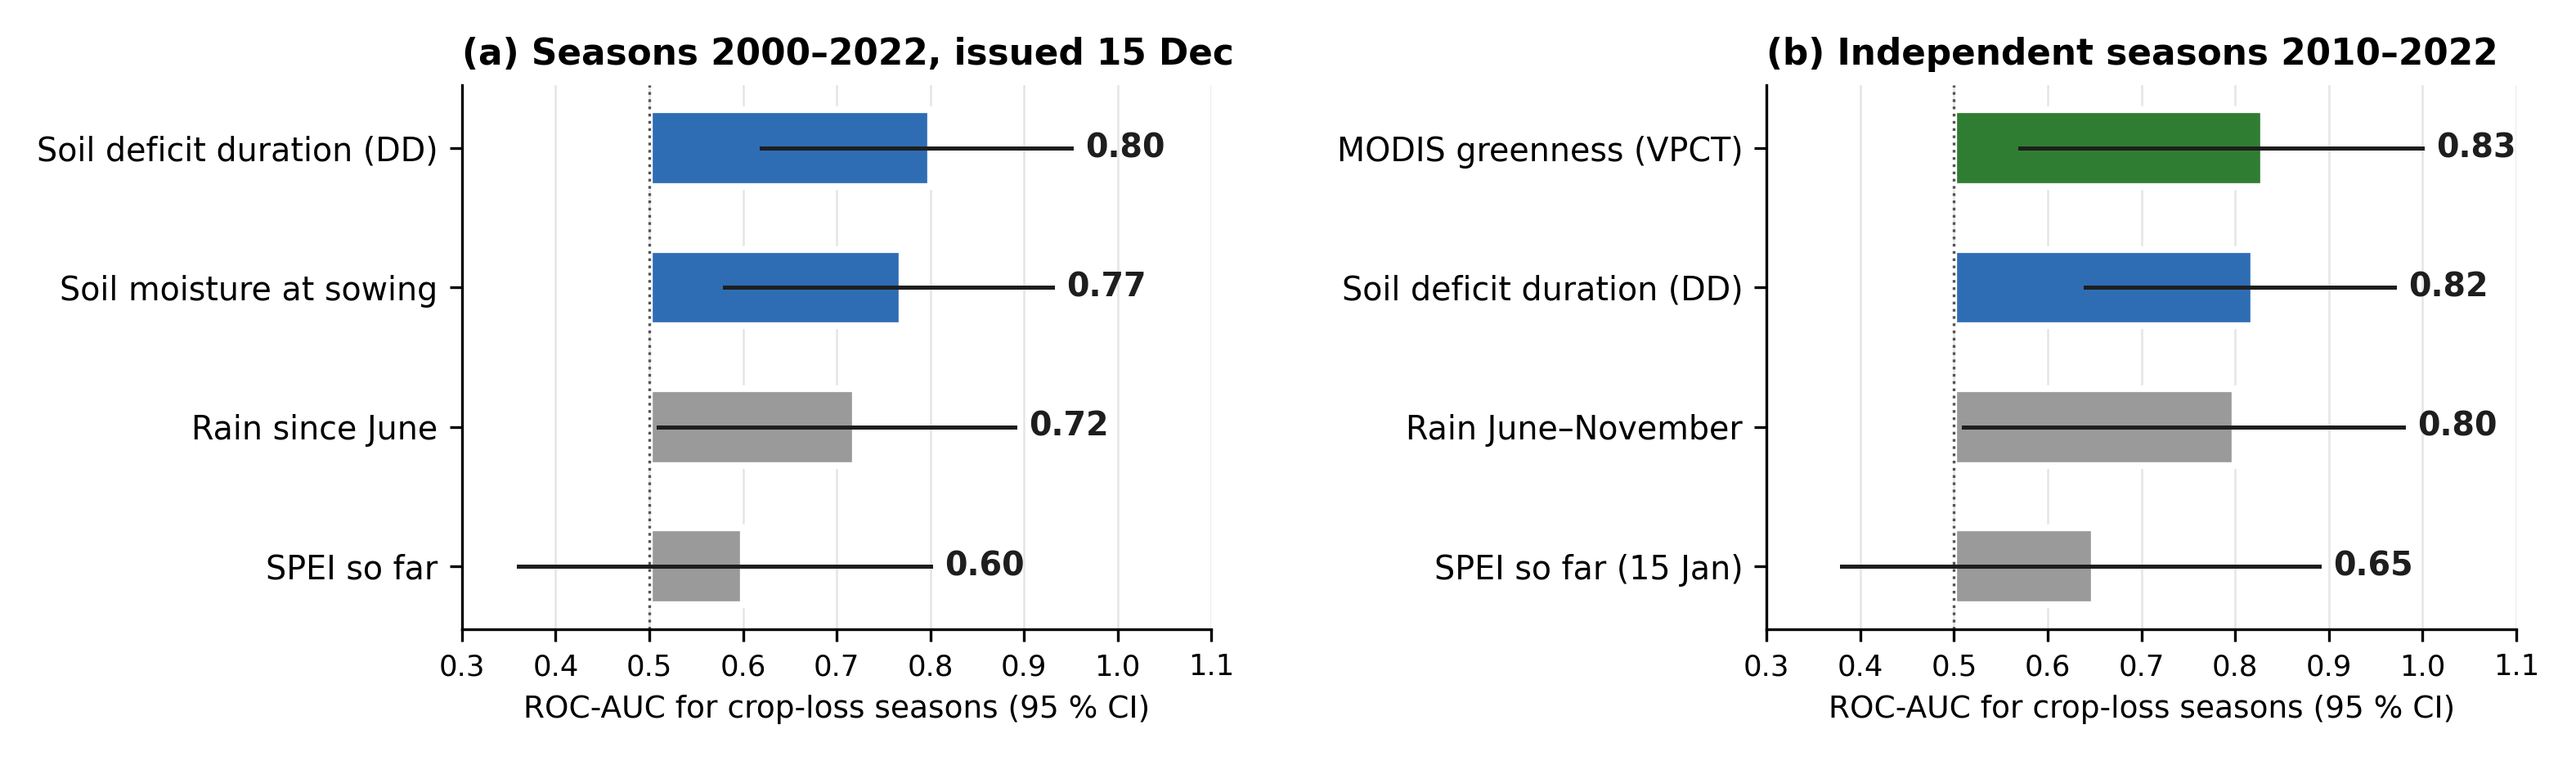
\includegraphics[width=0.98\textwidth]{figures/rabi_auc.png}\\[4pt]
  \begin{itemize}
    \item Soil drought indicator warns by \alert{15 December} (AUC 0.80); rain-based SPEI only 0.60
    \item MODIS greenness confirms it on 13 independent seasons (AUC 0.83)
  \end{itemize}
\end{frame}

\begin{frame}{Rabi: field early-drying warnings (30 days ahead)}
  \begin{columns}[c]
    \column{0.48\textwidth}
    \begin{itemize}
      \item Random forest on 1,350 Sentinel-2 points
      \item Warns of early drying up to \alert{30 days} ahead
      \item Each warning checked against soil moisture
    \end{itemize}
    \column{0.5\textwidth}
    \bignum{0.69 vs 0.56}{precision with vs without\\the soil check}
    \bignum{2$\times$}{warnings under dry soil are\\twice as often correct}
  \end{columns}
  \vspace{2pt}
  \hint{Test seasons 2023--2025; only 2023 was a dry season, so this is descriptive.}
\end{frame}

% ============================================================================
\section{UAV module}

\begin{frame}{UAV module: from drone photo to field report}
  \centering
  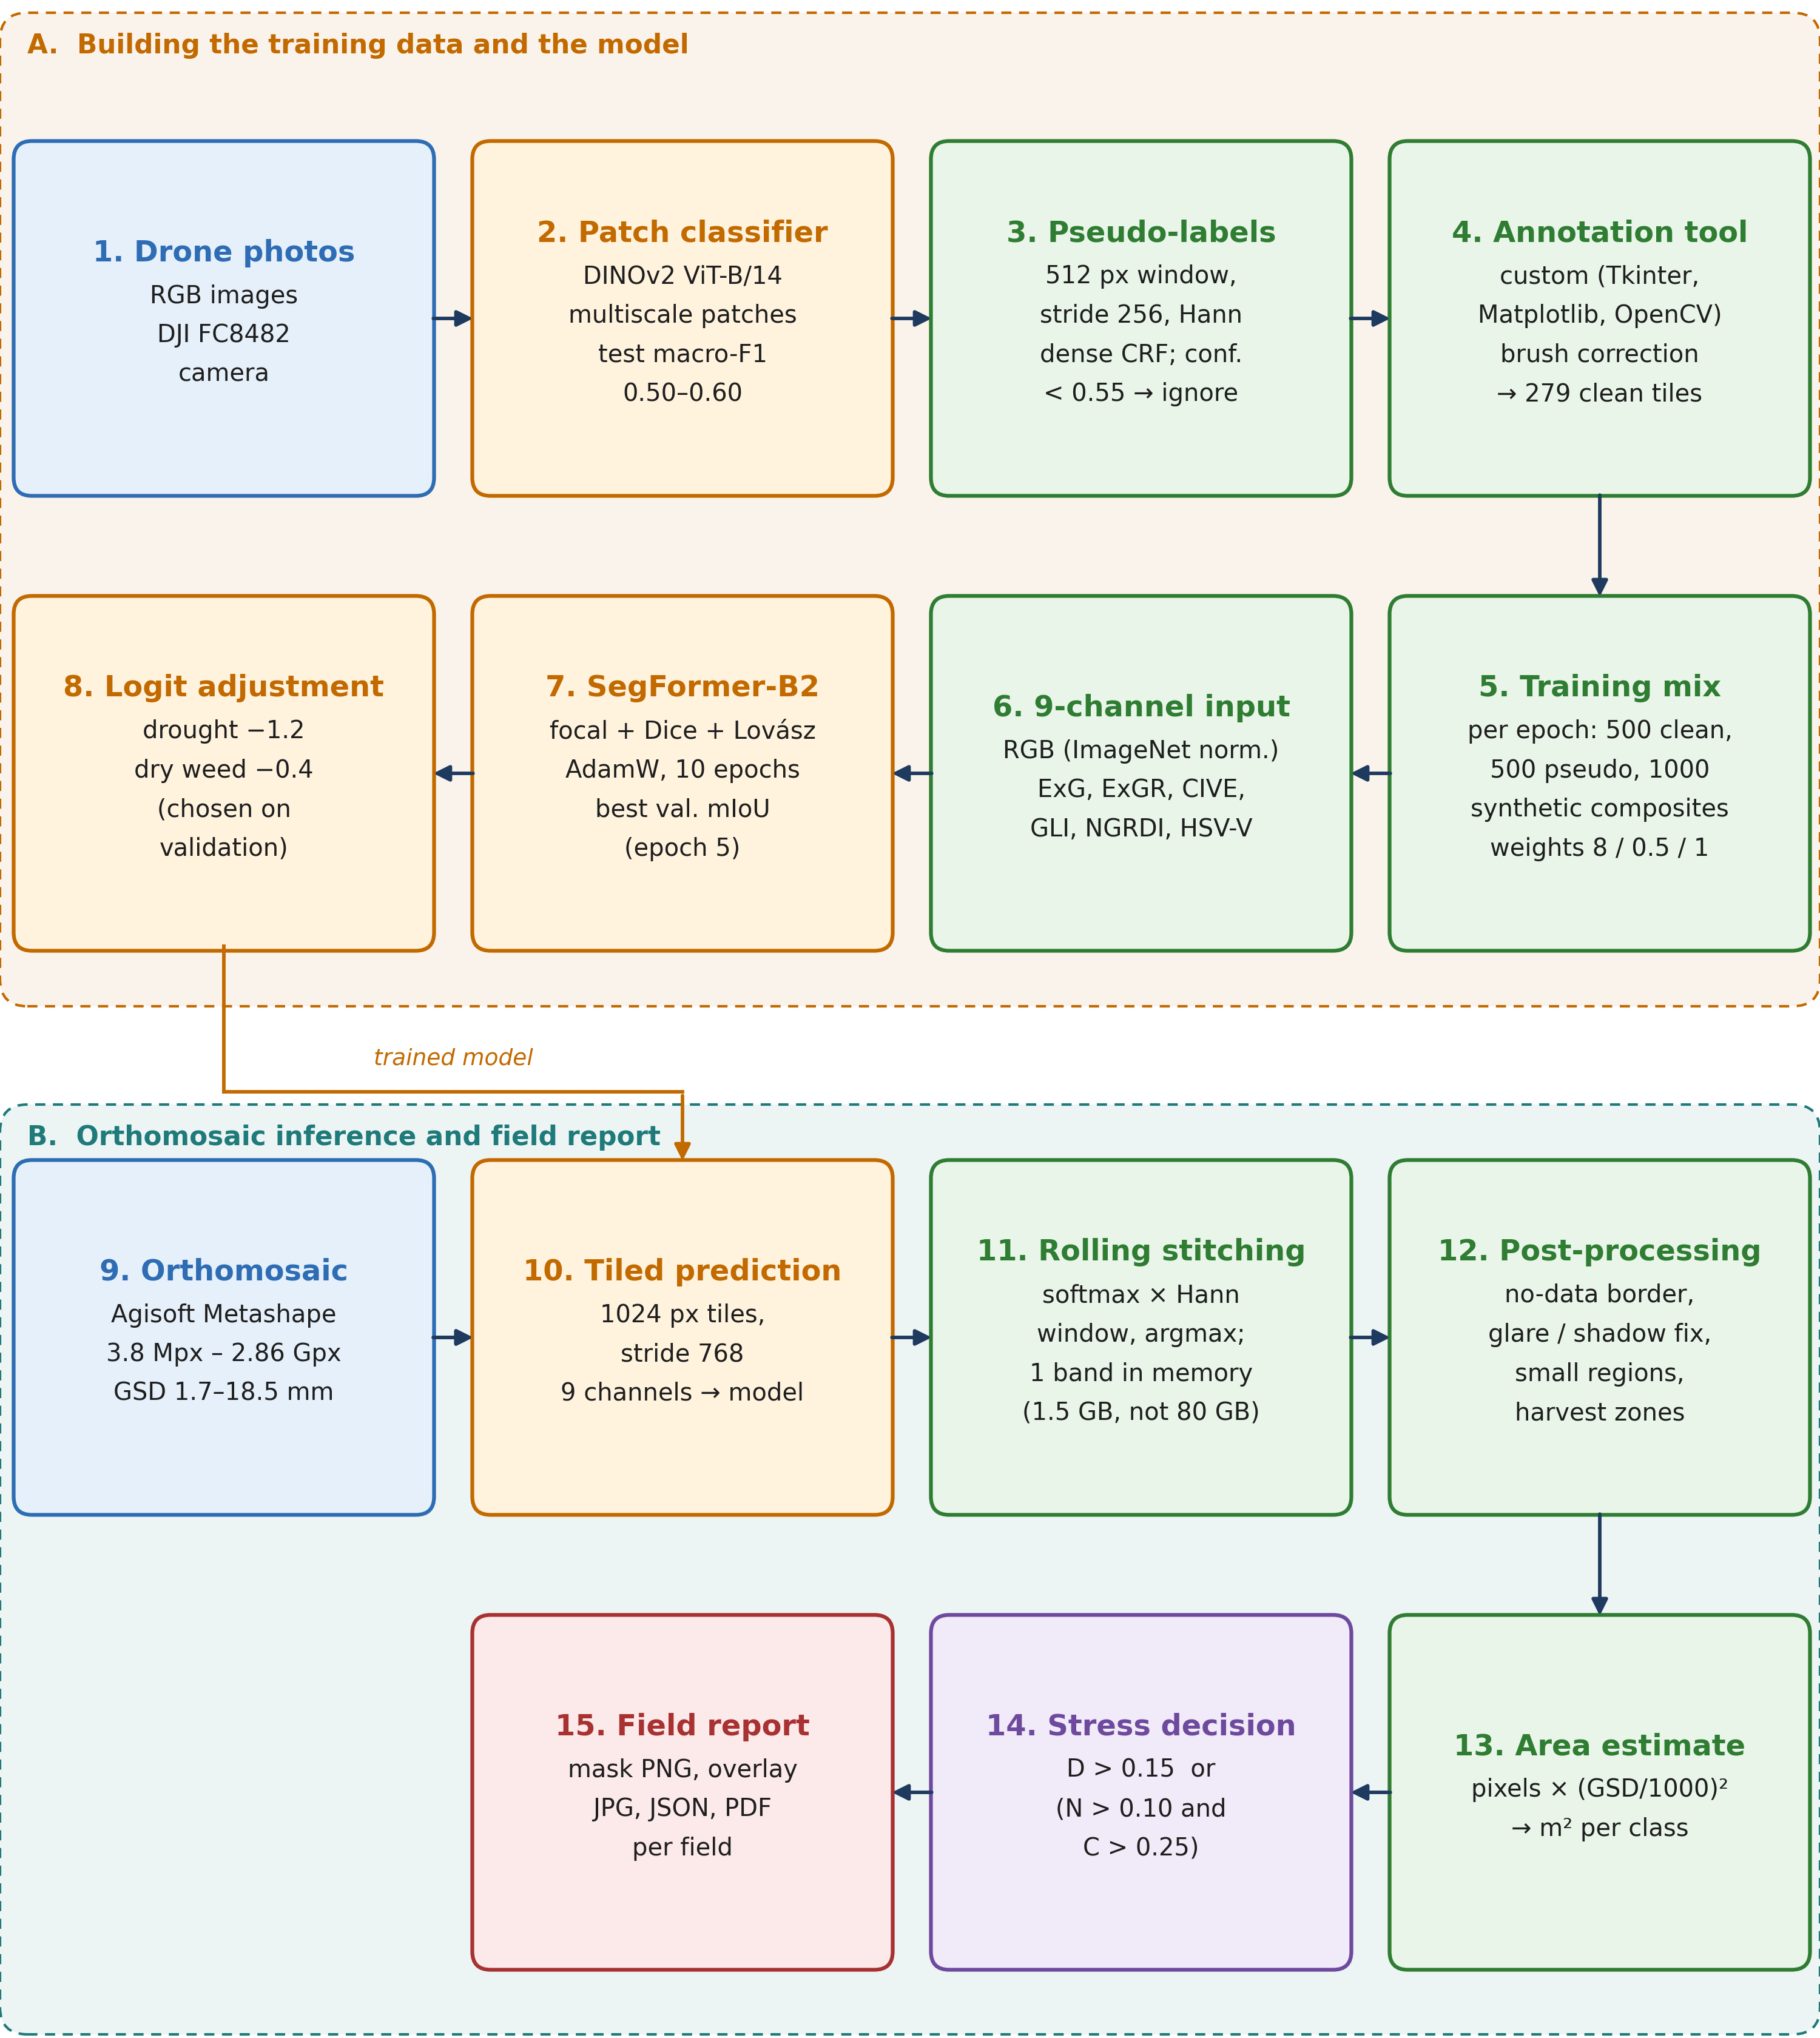
\includegraphics[height=0.84\textheight]{figures/v2_uav_pipeline.png}
\end{frame}

\begin{frame}{Step 1--4: building the labels}
  \centering
  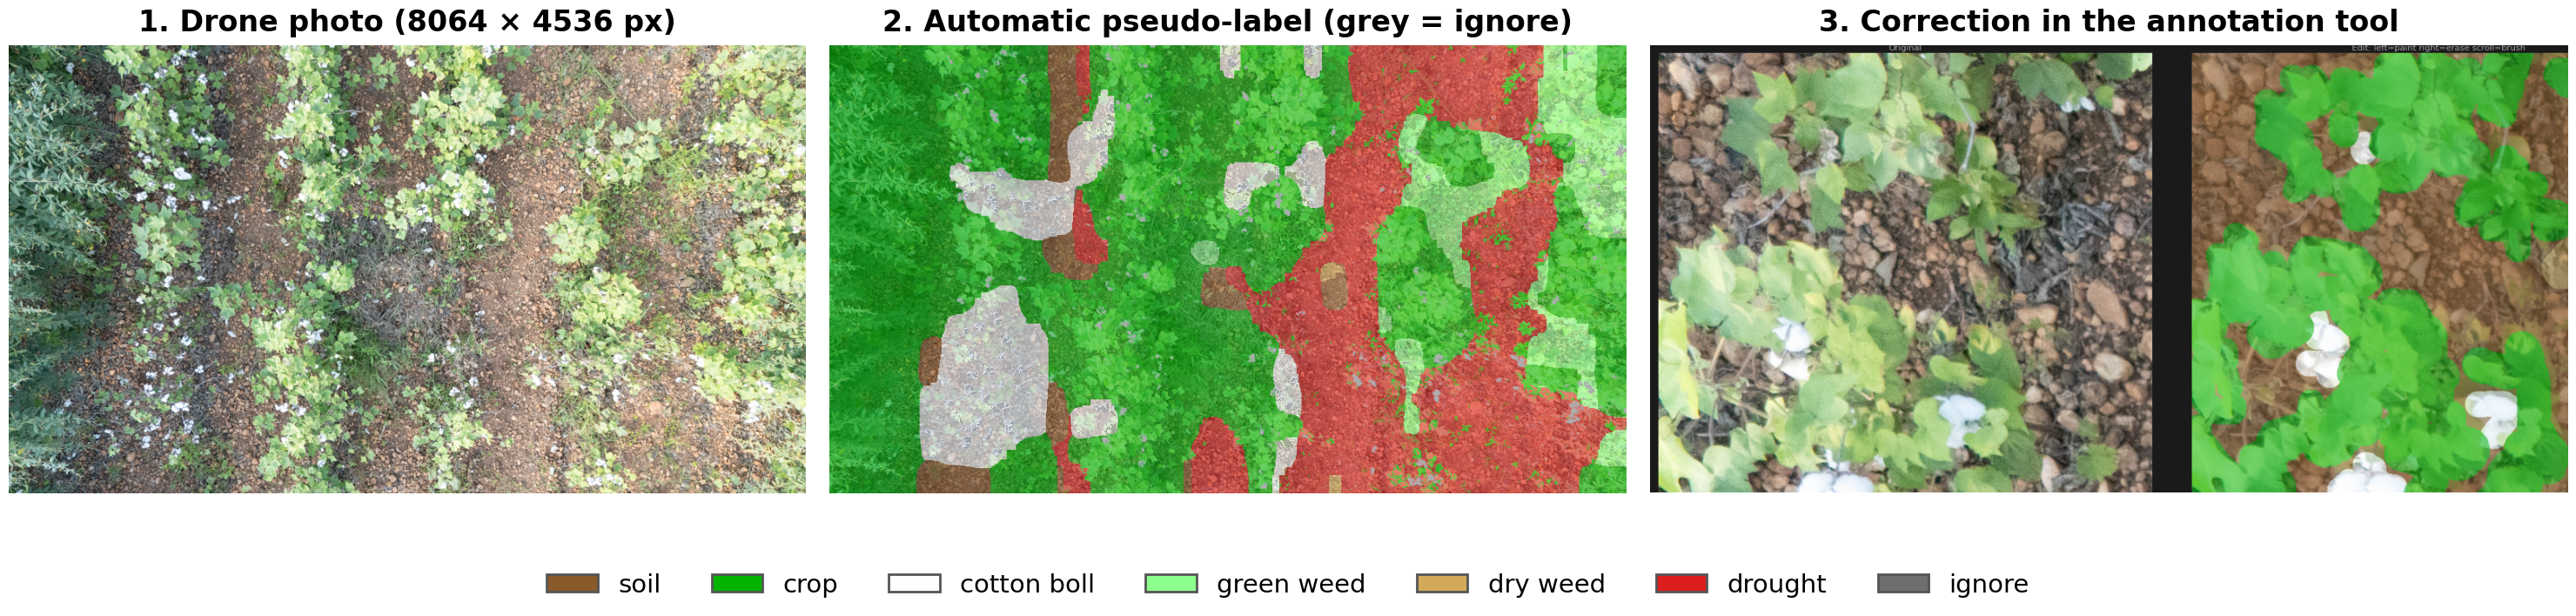
\includegraphics[width=\textwidth]{figures/uav_step_labels.png}\\[4pt]
  \begin{itemize}
    \item Automatic pseudo-labels are rough $\rightarrow$ corrected by hand in our \alert{own annotation tool}
    \item Result: \alert{279 clean tiles} (224 training, 55 validation)
  \end{itemize}
\end{frame}

\begin{frame}{Step 6: nine input channels}
  \centering
  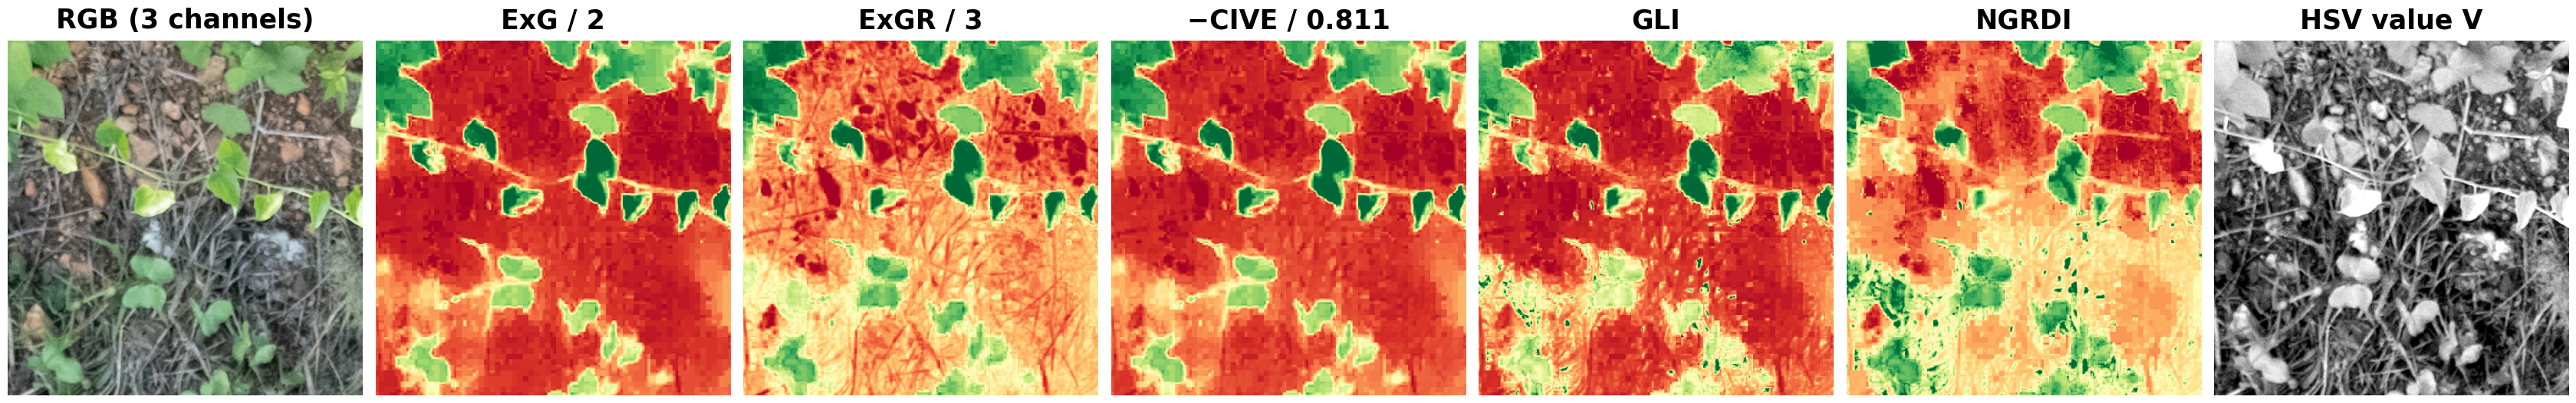
\includegraphics[width=\textwidth]{figures/uav_step_channels.png}\\[6pt]
  \begin{itemize}
    \item RGB + 5 vegetation indices + brightness
    \item Indices separate green leaves from soil and dry material much more sharply than RGB alone
  \end{itemize}
\end{frame}

\begin{frame}{Step 7: the model --- SegFormer-B2}
  \begin{columns}[c]
    \column{0.64\textwidth}
    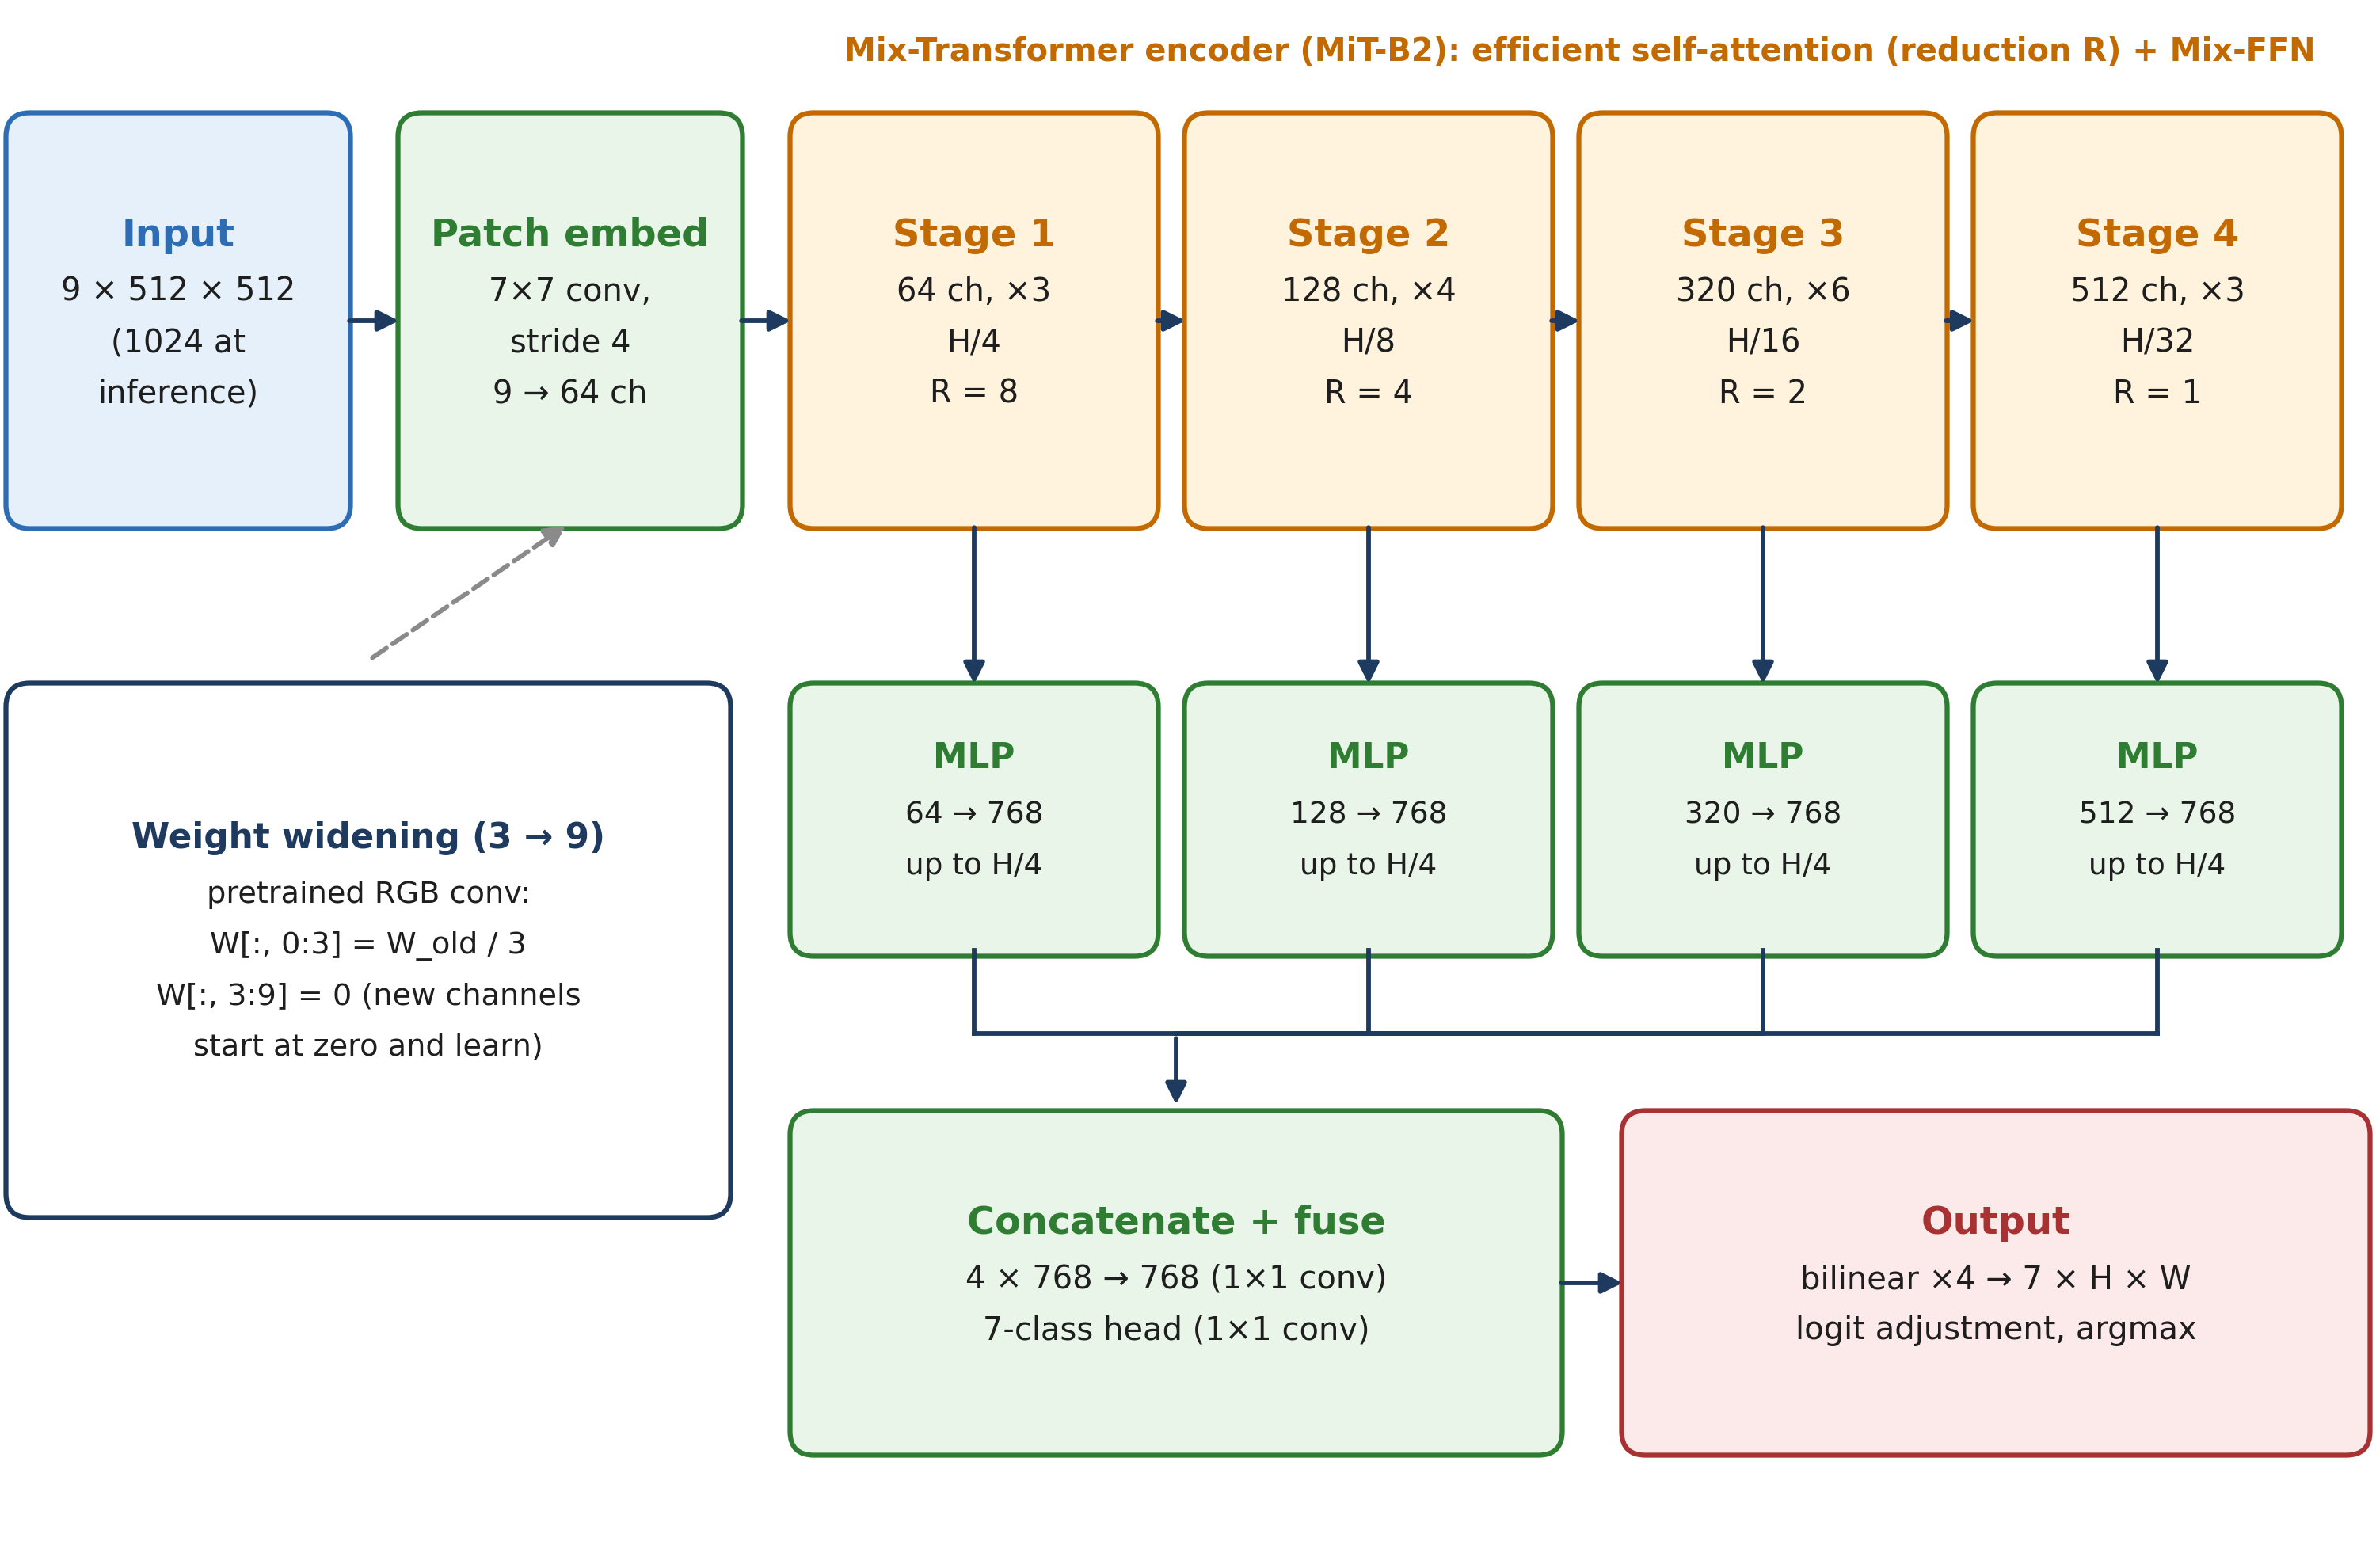
\includegraphics[width=\textwidth]{figures/v2_uav_model.png}
    \column{0.34\textwidth}
    \begin{itemize}
      \item Transformer encoder, 4 scales
      \item Input widened from 3 to \alert{9 channels}
      \item \alert{7 classes}: soil, crop, cotton boll, green weed, dry weed, drought, background
    \end{itemize}
  \end{columns}
\end{frame}

\begin{frame}{Step 10--11: how prediction stitching works}
  \centering
  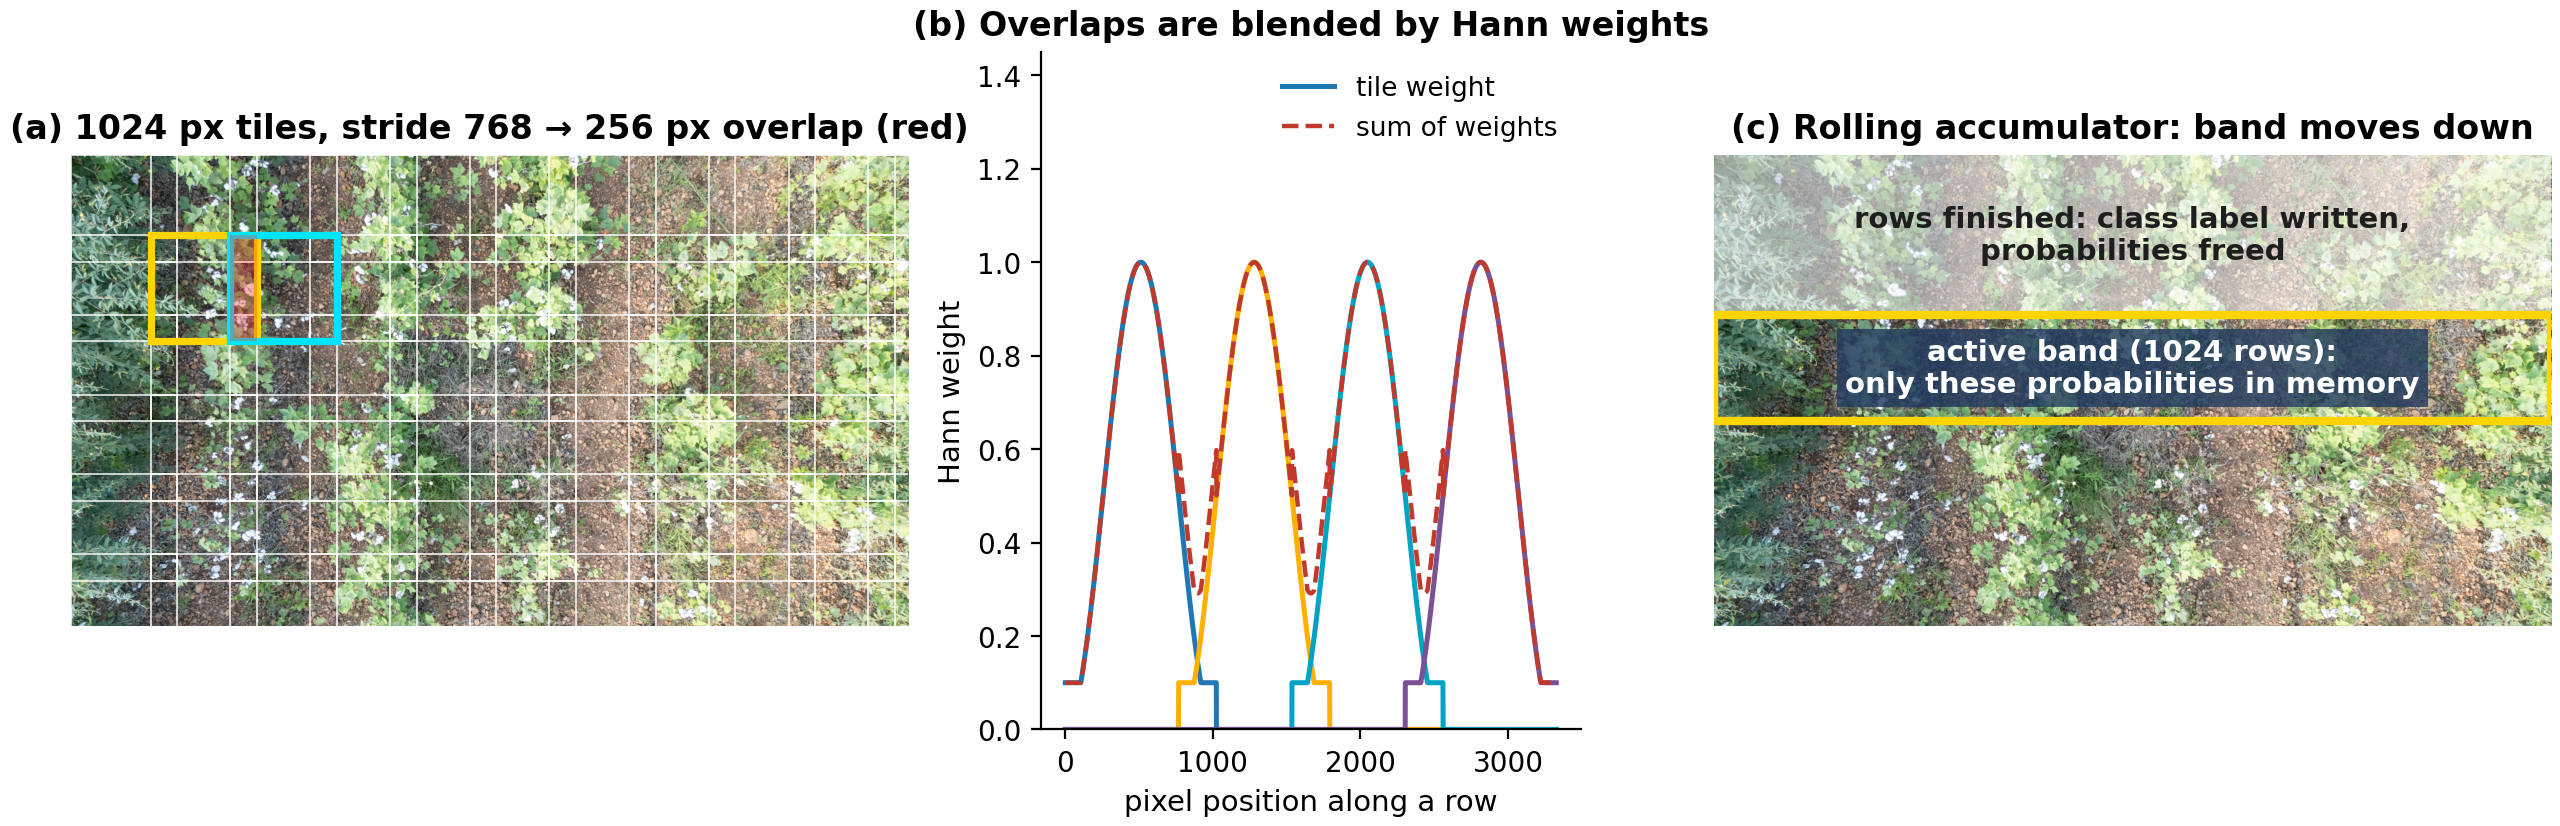
\includegraphics[width=\textwidth]{figures/uav_step_stitching.png}\\[4pt]
  \begin{itemize}
    \item Overlapping tiles + Hann weights $\rightarrow$ \alert{no seams} at tile borders
    \item Only one band in memory: \alert{1.5\,GB instead of 80\,GB} for a 2.9-billion-pixel orthomosaic
  \end{itemize}
\end{frame}

\begin{frame}{UAV results (55 validation tiles)}
  \begin{columns}[c]
    \column{0.36\textwidth}
    \bignum{65.1\,\%}{mIoU}
    \bignum{82.7\,\%}{pixel accuracy}
    \bignum{79.2\,\%}{drought F1}
    \column{0.6\textwidth}
    \centering
    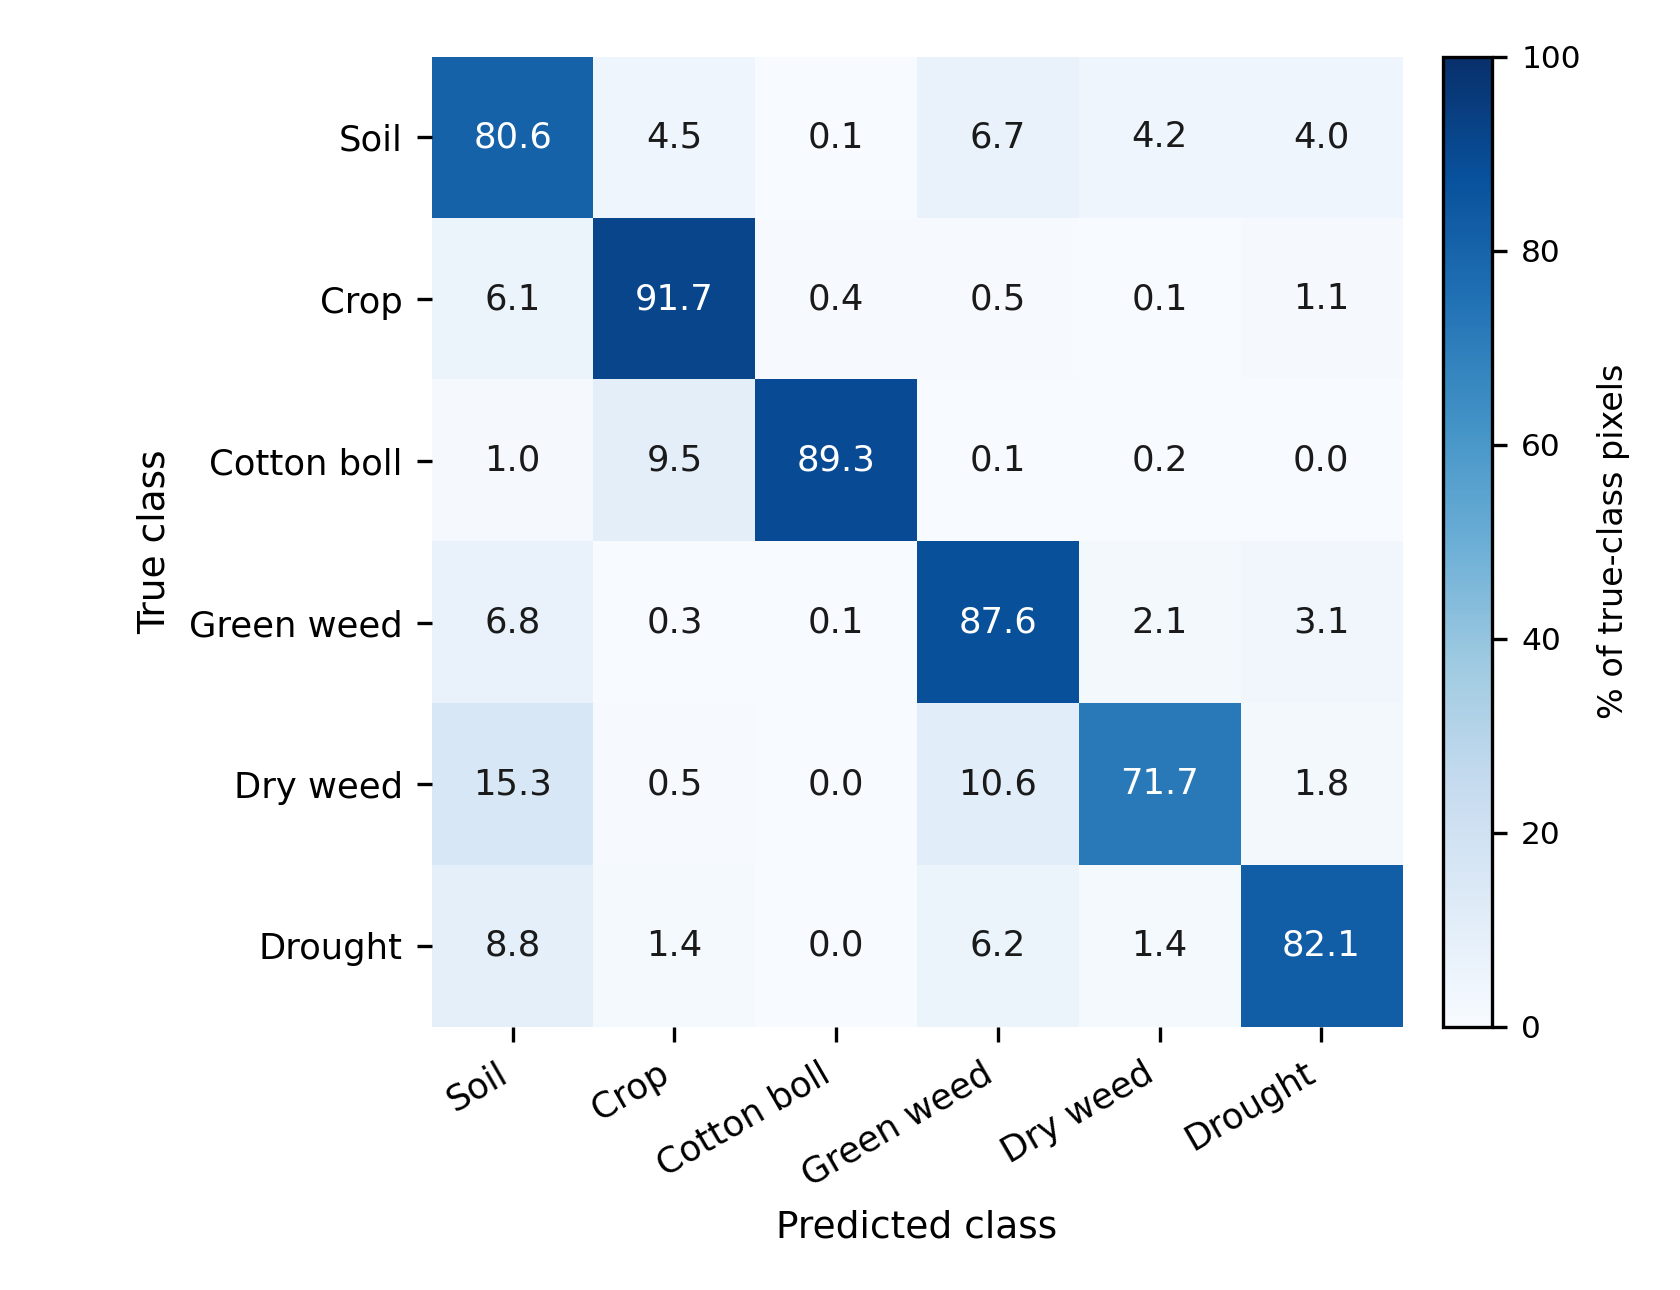
\includegraphics[height=0.68\textheight]{figures/uav_confusion.png}\\
    \hint{Validation, not an independent test; drought / dry-weed adjustment chosen on these tiles.}
  \end{columns}
\end{frame}

\begin{frame}{UAV results on real fields}
  \begin{columns}[c]
    \column{0.5\textwidth}
    \centering
    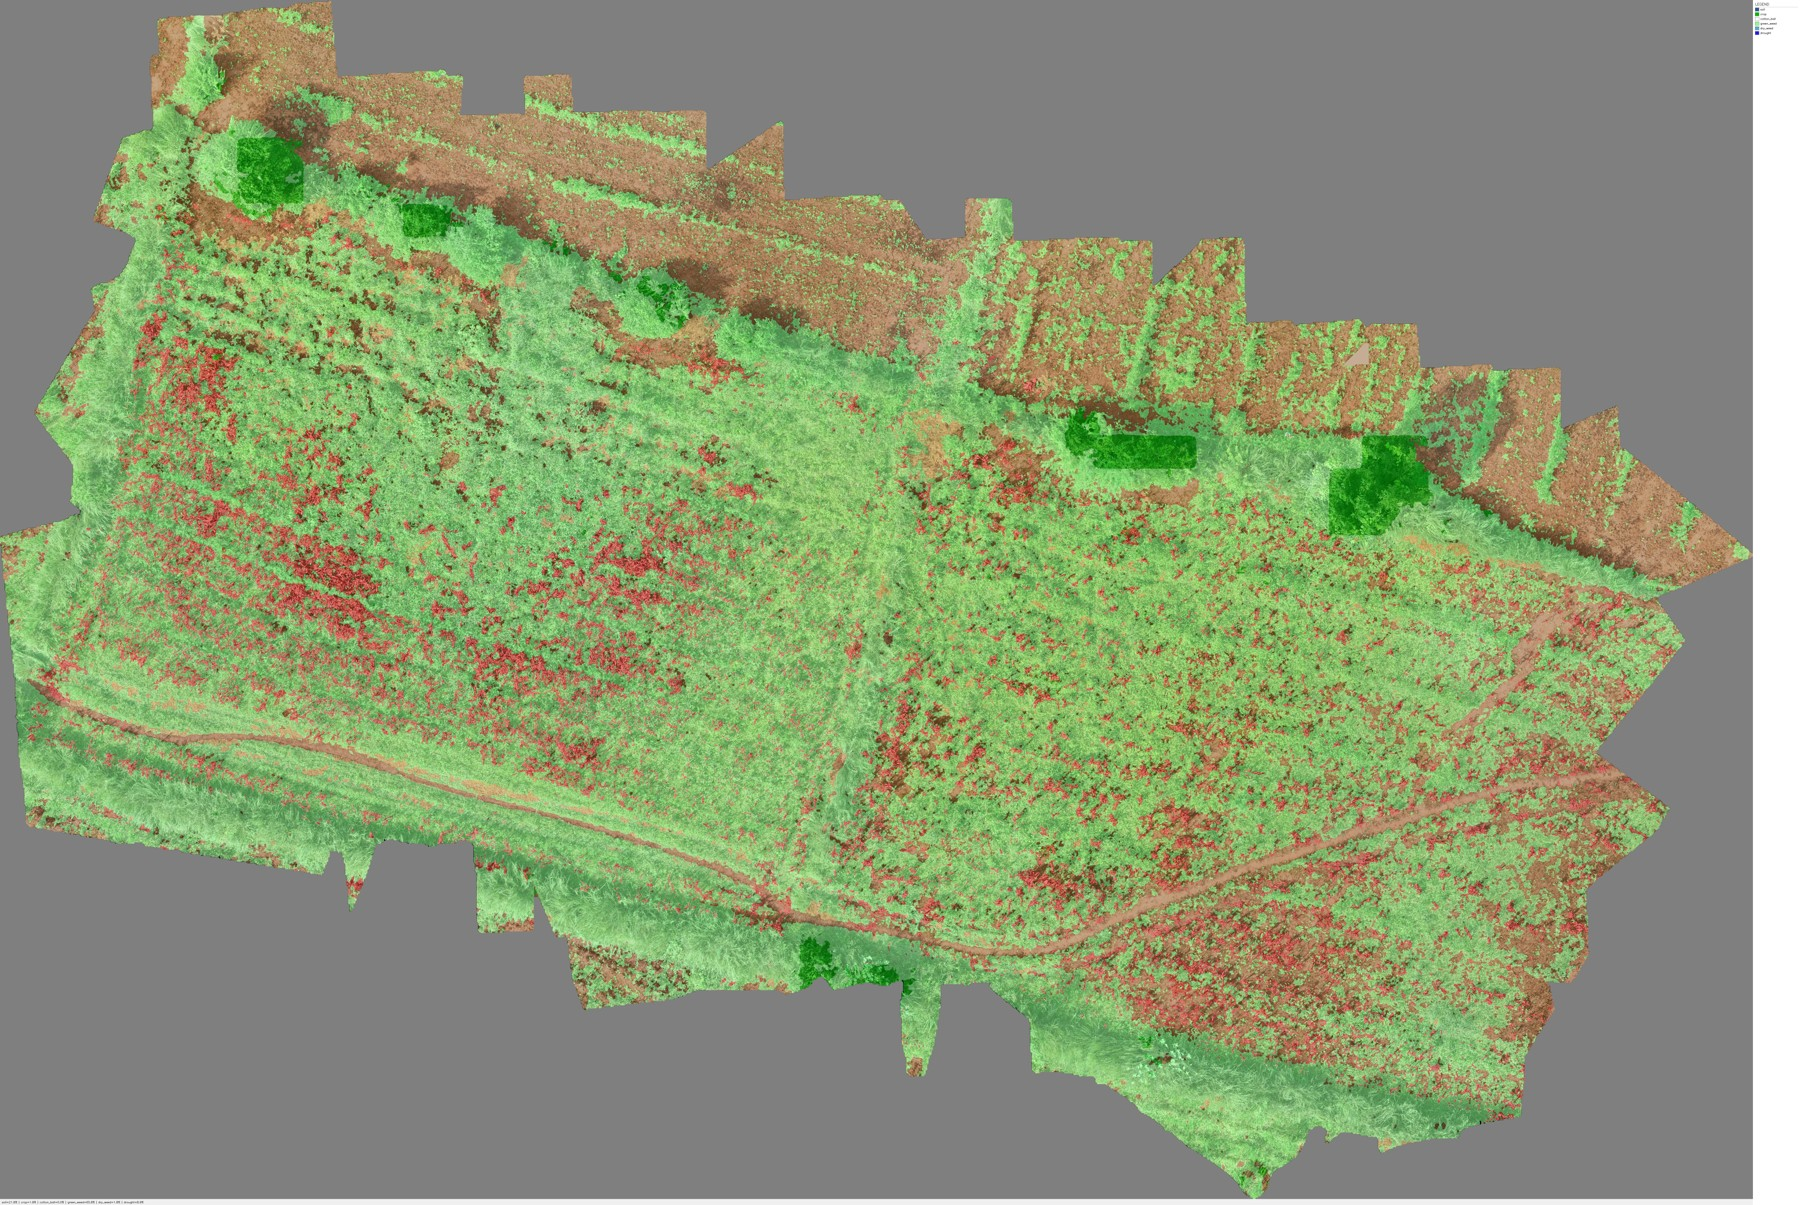
\includegraphics[width=\textwidth]{figures/uav_lepakshi_overlay.jpg}\\
    \hint{Lepakshi: 71.5\,\% drought (red) $\rightarrow$ flagged}
    \column{0.22\textwidth}
    \centering
    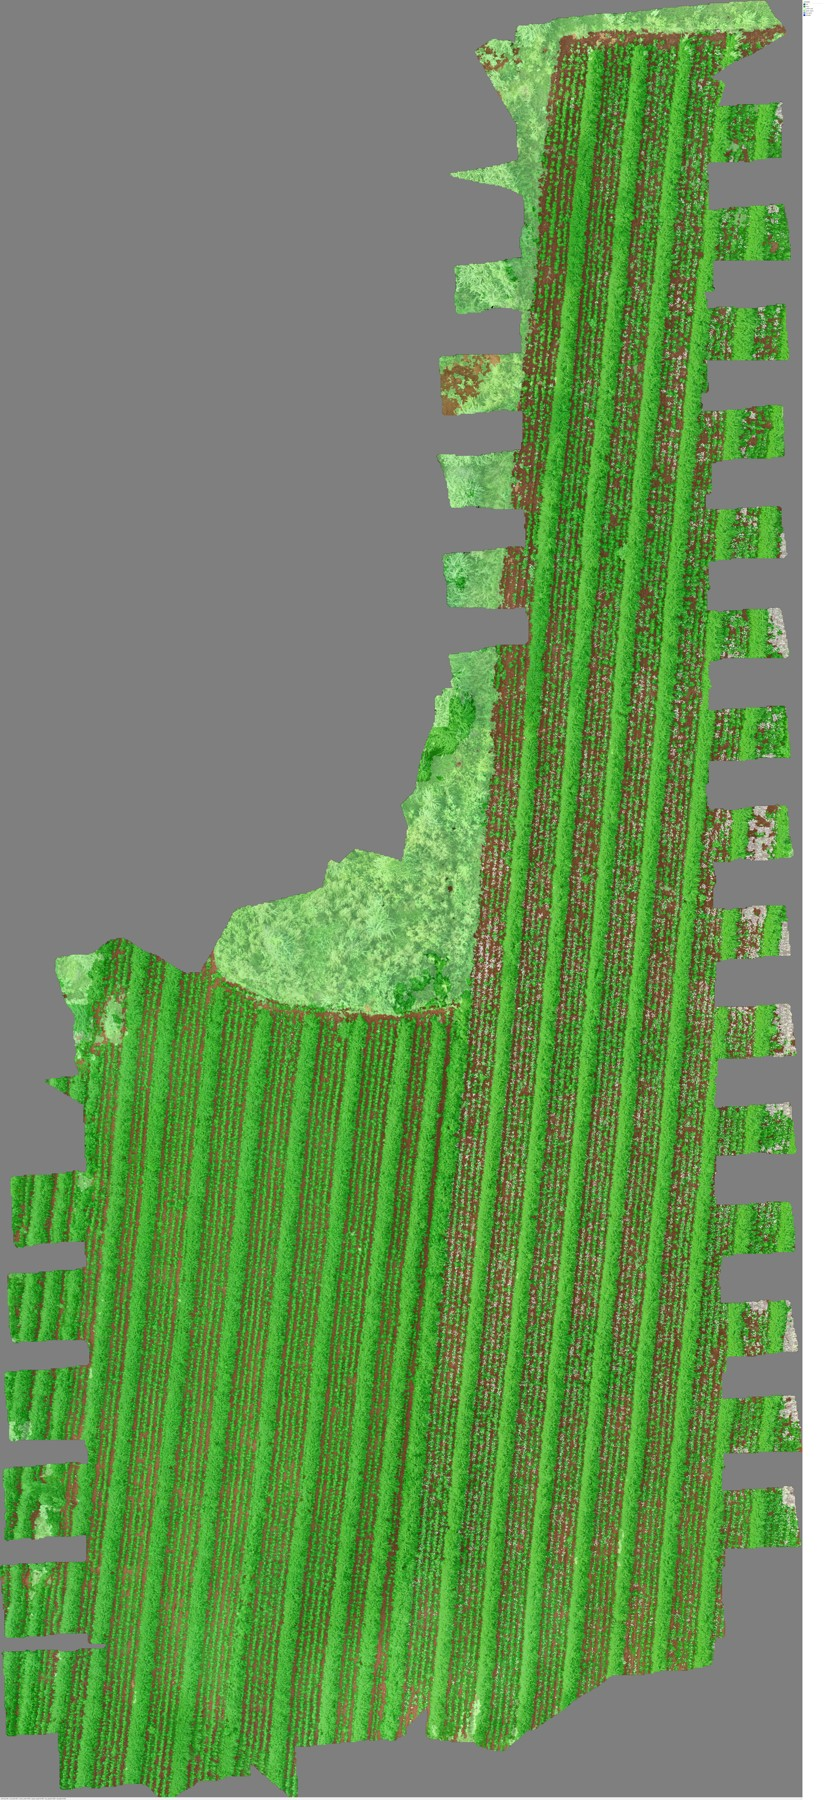
\includegraphics[height=0.6\textheight]{figures/uav_knlddp_overlay.jpg}\\
    \hint{KNL cotton: not flagged}
    \column{0.26\textwidth}
    \bignum{3 of 14}{fields flagged --- the same southern maize fields the survey team judged drought-hit}
  \end{columns}
\end{frame}

% ============================================================================
\section{Conclusion}

\begin{frame}{Summary}
  \begin{columns}[T]
    \column{0.32\textwidth}
    \begin{block}{Kharif}
      \centering
      {\Large\bfseries\color{amber}9 / 9}\\severe droughts confirmed\\(5 before the order)
    \end{block}
    \column{0.32\textwidth}
    \begin{block}{Rabi}
      \centering
      {\Large\bfseries\color{amber}AUC 0.80}\\crop-loss warning\\by 15 December
    \end{block}
    \column{0.32\textwidth}
    \begin{block}{UAV}
      \centering
      {\Large\bfseries\color{amber}65.1\,\% mIoU}\\7-class maps of\\2.9-billion-pixel fields
    \end{block}
  \end{columns}
  \vspace{10pt}
  \begin{itemize}
    \item Kharif and rabi modules \alert{hand stressed fields to the drone}
  \end{itemize}
\end{frame}

\begin{frame}{Limitations and future work}
  \begin{columns}[T]
    \column{0.48\textwidth}
    \textbf{Limitations}
    \begin{itemize}
      \item No field-level ground truth yet
      \item No skill 30 days ahead (kharif)
      \item Few dry rabi seasons in the test
      \item UAV: validation only, not an independent test
    \end{itemize}
    \column{0.48\textwidth}
    \textbf{Future work}
    \begin{itemize}
      \item Run the full loop in rabi 2026-27
      \item Finish the 127-tile independent UAV test
      \item Multispectral / thermal drone imagery
    \end{itemize}
  \end{columns}
\end{frame}

\begin{frame}{Key references}
  \footnotesize
  \begin{itemize}
    \item Vicente-Serrano et al., \emph{SPEI drought index}, J.\ Climate, 2010
    \item Marusov et al., \emph{Drought prediction with deep networks}, Environ.\ Model.\ Softw., 2024
    \item Peters et al., \emph{Standardized Vegetation Index}, PE\&RS, 2002
    \item Bhardwaj \& Mishra, \emph{Drought detection and declaration in India}, Water Security, 2021
    \item Padhee et al., \emph{Rabi drought in Bundelkhand}, ISPRS Arch., 2014
    \item Xie et al., \emph{SegFormer}, NeurIPS, 2021
    \item Shahi et al., \emph{Cotton water stress from UAV images}, Remote Sens., 2023
  \end{itemize}
\end{frame}

\begin{frame}[standout]
  Thank you\\[6pt]
  {\normalsize Questions?}
\end{frame}

\end{document}
